% Copyright 2018-2022 FIUS
%
% This file is part of theo-vorkurs-folien.
%
% theo-vorkurs-folien is free software: you can redistribute it and/or modify
% it under the terms of the GNU General Public License as published by
% the Free Software Foundation, either version 3 of the License, or
% (at your option) any later version.
%
% theo-vorkurs-folien is distributed in the hope that it will be useful,
% but WITHOUT ANY WARRANTY; without even the implied warranty of
% MERCHANTABILITY or FITNESS FOR A PARTICULAR PURPOSE.  See the
% GNU General Public License for more details.
%
% You should have received a copy of the GNU General Public License
% along with theo-vorkurs-folien.  If not, see <https://www.gnu.org/licenses/>.

% !TeX program = pdflatex
% !TeX spellcheck = de
% Copyright 2018-2022 FIUS
%
% This file is part of theo-vorkurs-folien.
%
% theo-vorkurs-folien is free software: you can redistribute it and/or modify
% it under the terms of the GNU General Public License as published by
% the Free Software Foundation, either version 3 of the License, or
% (at your option) any later version.
%
% theo-vorkurs-folien is distributed in the hope that it will be useful,
% but WITHOUT ANY WARRANTY; without even the implied warranty of
% MERCHANTABILITY or FITNESS FOR A PARTICULAR PURPOSE.  See the
% GNU General Public License for more details.
%
% You should have received a copy of the GNU General Public License
% along with theo-vorkurs-folien.  If not, see <https://www.gnu.org/licenses/>.

\documentclass[aspectratio=43,10pt]{beamer}

\usetheme[progressbar=frametitle]{metropolis}
\usepackage{appendixnumberbeamer}
\usepackage[ngerman]{babel}
\usepackage[utf8]{inputenc}
%\usepackage{t1enc}
\usepackage[T1]{fontenc}
\usepackage[sfdefault,scaled=.85,lf]{FiraSans}
\usepackage{newtxsf}

\usepackage{booktabs}
\usepackage[scale=2]{ccicons}
\usepackage{hyperref}

\usepackage{pgf}
\makeatletter
\@ifclasswith{beamer}{notes}{
  \usepackage{pgfpages}
  \setbeameroption{show notes on second screen}
}{}
\makeatother
\usepackage{tikz}
\usetikzlibrary{arrows,automata,positioning}
\usepackage{pgfplots}
\usepgfplotslibrary{dateplot}

\usepackage{xspace}
\newcommand{\themename}{\textbf{\textsc{metropolis}}\xspace}

\usepackage{blindtext}
\usepackage{graphicx}
\usepackage{subcaption}
\usepackage{comment}
\usepackage{mathtools}
\usepackage{amsmath}
\usepackage{centernot}
\usepackage{amssymb}
\usepackage{proof}
\usepackage{tabularx}
\renewcommand{\figurename}{Abb.}
\usepackage{marvosym}
\usepackage{mathtools}
\usepackage{qrcode}
\usepackage{advdate}

\newcommand\daynr{0}

\definecolor{ExColor}{HTML}{17819b}

\newcommand{\emptyWord}{\varepsilon}
\let \emptyset\varnothing
\newcommand{\SigmaStern}{\Sigma^{*}}
\newcommand{\absval}[1]{|#1|}
\newcommand{\defeq}{\vcentcolon=}
\newcommand{\eqdef}{=\vcentcolon}
\newcommand{\nimplies}{\centernot\implies}

\newcommand{\naturals}{\ensuremath{\mathbb{N}}}
\newcommand{\integers}{\ensuremath{\mathbb{Z}}}
\newcommand{\rationals}{\ensuremath{\mathbb{Q}}}
\newcommand{\reals}{\ensuremath{\mathbb{R}}}
\newcommand{\iffspace}{\ensuremath{\iff\;}}

\setbeamertemplate{footline}[text line]
{\parbox{\linewidth}{Fachgruppe Informatik\hfill\insertpagenumber\hfill Vorkurs Theoretische Informatik\vspace{0.2in}}}

\newcommand{\Center}[1]{
  \begin{frame}<handout:0>[standout]
    #1
  \end{frame}
}

% Fix section pages in appendix
\AtBeginDocument{%
  \apptocmd{\appendix}{%
    \setbeamertemplate{section page}[simple]%
  }{}{}
}

\addtobeamertemplate{block begin}{}{\vskip 0em}
\addtobeamertemplate{block alerted begin}{}{\vskip 0em}
\addtobeamertemplate{block example begin}{}{\vskip 0em}

% Copyright 2018-2022 FIUS
%
% This file is part of theo-vorkurs-folien.
%
% theo-vorkurs-folien is free software: you can redistribute it and/or modify
% it under the terms of the GNU General Public License as published by
% the Free Software Foundation, either version 3 of the License, or
% (at your option) any later version.
%
% theo-vorkurs-folien is distributed in the hope that it will be useful,
% but WITHOUT ANY WARRANTY; without even the implied warranty of
% MERCHANTABILITY or FITNESS FOR A PARTICULAR PURPOSE.  See the
% GNU General Public License for more details.
%
% You should have received a copy of the GNU General Public License
% along with theo-vorkurs-folien.  If not, see <https://www.gnu.org/licenses/>.



% Configuration for slides

% The date of the first day of the Theo-Vorkurs in Format dd/mm/yyyy
\SetDate[10/10/2022]

% Invite URL to the Ersti-Telegram-Group. Used for text on slide as well as QR-Code
\newcommand\telegramurl{https://t.me/+Q92w5biyY903NjEy}

% The url to the handout of the current day with the current day as argument. Used for the qr-code in the slides. 
\newcommand{\handouturl}[1]{https://fius.de/wp-content/uploads/2022/10/day-#1-handout.pdf}


\renewcommand\daynr{3}
% Copyright 2018-2022 FIUS
%
% This file is part of theo-vorkurs-folien.
%
% theo-vorkurs-folien is free software: you can redistribute it and/or modify
% it under the terms of the GNU General Public License as published by
% the Free Software Foundation, either version 3 of the License, or
% (at your option) any later version.
%
% theo-vorkurs-folien is distributed in the hope that it will be useful,
% but WITHOUT ANY WARRANTY; without even the implied warranty of
% MERCHANTABILITY or FITNESS FOR A PARTICULAR PURPOSE.  See the
% GNU General Public License for more details.
%
% You should have received a copy of the GNU General Public License
% along with theo-vorkurs-folien.  If not, see <https://www.gnu.org/licenses/>.

\title{Vorkurs Theoretische Informatik}

\if\daynr1
    \subtitle{Einführung in die Grundideen, Mengenlehre und Aussagenlogik}
    \newcommand\daynamestr{Montag}
\fi
\if\daynr2
    \subtitle{Grundlagen der Beweise}
    \newcommand\daynamestr{Dienstag}
    \AdvanceDate
\fi
\if\daynr3
    \subtitle{Induktion und Einführung in die Grammatik}
    \newcommand\daynamestr{Mittwoch}
    \AdvanceDate\AdvanceDate
\fi
\if\daynr4
    \subtitle{Einführung in reguläre Sprachen}
    \newcommand\daynamestr{Donnerstag}
    \AdvanceDate\AdvanceDate\AdvanceDate
\fi
\if\daynr5
    \subtitle{Einführung in reguläre Sprachen}
    \newcommand\daynamestr{Freitag}
    \AdvanceDate\AdvanceDate\AdvanceDate
\fi


\date{\daynamestr, \today}

\author{Arbeitskreis Theo-Vorkurs}
\institute{Fachgruppe Informatik}
% \titlegraphic{\hfill\includegraphics[height=1.5cm]{logo.pdf}}

\begin{document}

\maketitle

\begin{frame}[fragile]{Übersicht}
    \setbeamertemplate{section in toc}[sections numbered]
    \tableofcontents%[hideallsubsections]
\end{frame}

\section{Vollständige Induktion}

% Copyright 2018-2022 FIUS
%
% This file is part of theo-vorkurs-folien.
%
% theo-vorkurs-folien is free software: you can redistribute it and/or modify
% it under the terms of the GNU General Public License as published by
% the Free Software Foundation, either version 3 of the License, or
% (at your option) any later version.
%
% theo-vorkurs-folien is distributed in the hope that it will be useful,
% but WITHOUT ANY WARRANTY; without even the implied warranty of
% MERCHANTABILITY or FITNESS FOR A PARTICULAR PURPOSE.  See the
% GNU General Public License for more details.
%
% You should have received a copy of the GNU General Public License
% along with theo-vorkurs-folien.  If not, see <https://www.gnu.org/licenses/>.

\begin{frame}[fragile]{Idee}
    \begin{columns}
        \column{0.5\textwidth}
        \begin{alertblock}{Zeige Aussagen der Form:\\\emph{Für alle $n\in\mathbb{N}$ gilt\ldots}}
            \begin{enumerate}
                \item Zeige Aussage für das kleinste Element
                \item<1-> \only<7,8|handout:0>{\alert<7>{Zeige, wenn Aussage für beliebiges $n$ gilt, gilt sie auch für dessen Nachfolger, also $n+1$.}}\onslide<1-6>{Zeige, dass Aussage auch für das folgende Element gilt.}
                \item<2-6,8> \only<8|handout:0>{\alert<8>{$\leadsto$ Aussage gilt für alle $n$.}}\onslide<2-6>{\small Zeige, dass Aussage auch für das folgende Element gilt.}
                \item<3-6> \footnotesize Zeige, dass Aussage auch für das folgende Element gilt.
                \item<4-6> \scriptsize Zeige, dass Aussage auch für das folgende Element gilt.
                \item<5-6> \tiny Zeige, dass Aussage auch für das folgende Element gilt.
                \item<6> \dots
            \end{enumerate}
        \end{alertblock}
        \column{0.5\textwidth}
        \begin{figure}
            \centering
            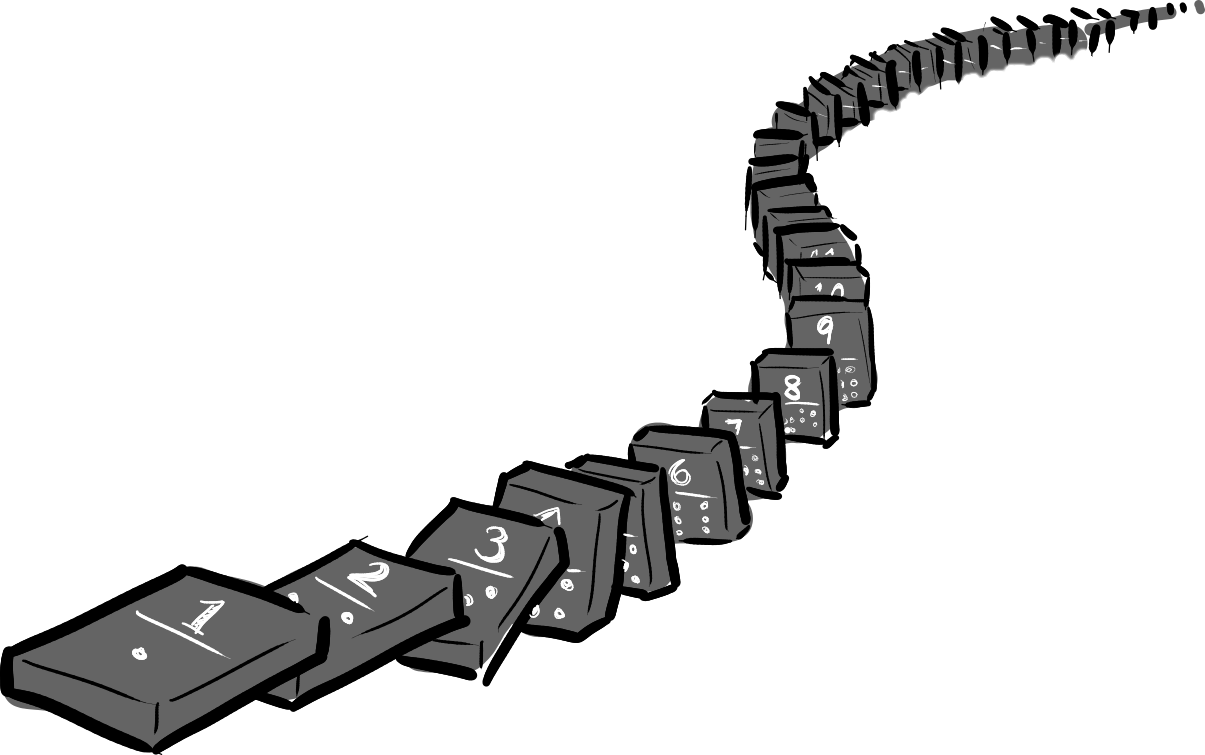
\includegraphics[width=0.7\textwidth]{../figures/induction.png}
            %\caption{Idee}
            %
        \end{figure}
    \end{columns}
\end{frame}

\subsection{Funktionsweise}
\begin{frame}[fragile]{Struktur}
    \begin{alertblock}{Zeige Aussagen der Form:\\\emph{Für alle $n\in\mathbb{N}$ gilt\ldots}}
        \begin{enumerate}
            \item \alert{Induktionsanfang}\\Zeige Aussage für das kleinste Element
            \item \alert{Induktionsvoraussetzung}\\Zeige, unter der Voraussetzung: \\\emph{die Aussage gelte für beliebiges $n$},\dots
            \item \alert{Induktionsschritt}\\\dots dann gilt die Aussage auch für dessen Nachfolger $n+1$.
            \item $\leadsto$ Aussage gilt für alle $n \in \mathbb{N}$.
        \end{enumerate}
    \end{alertblock}
\end{frame}

\begin{frame}[fragile]{Beispiel}
    \center $\displaystyle\sum_{i = 0}^{n} (2i+1) = (n+1)^2,\quad\forall n \in\mathbb{N}$.
    \begin{figure}
        \centering
        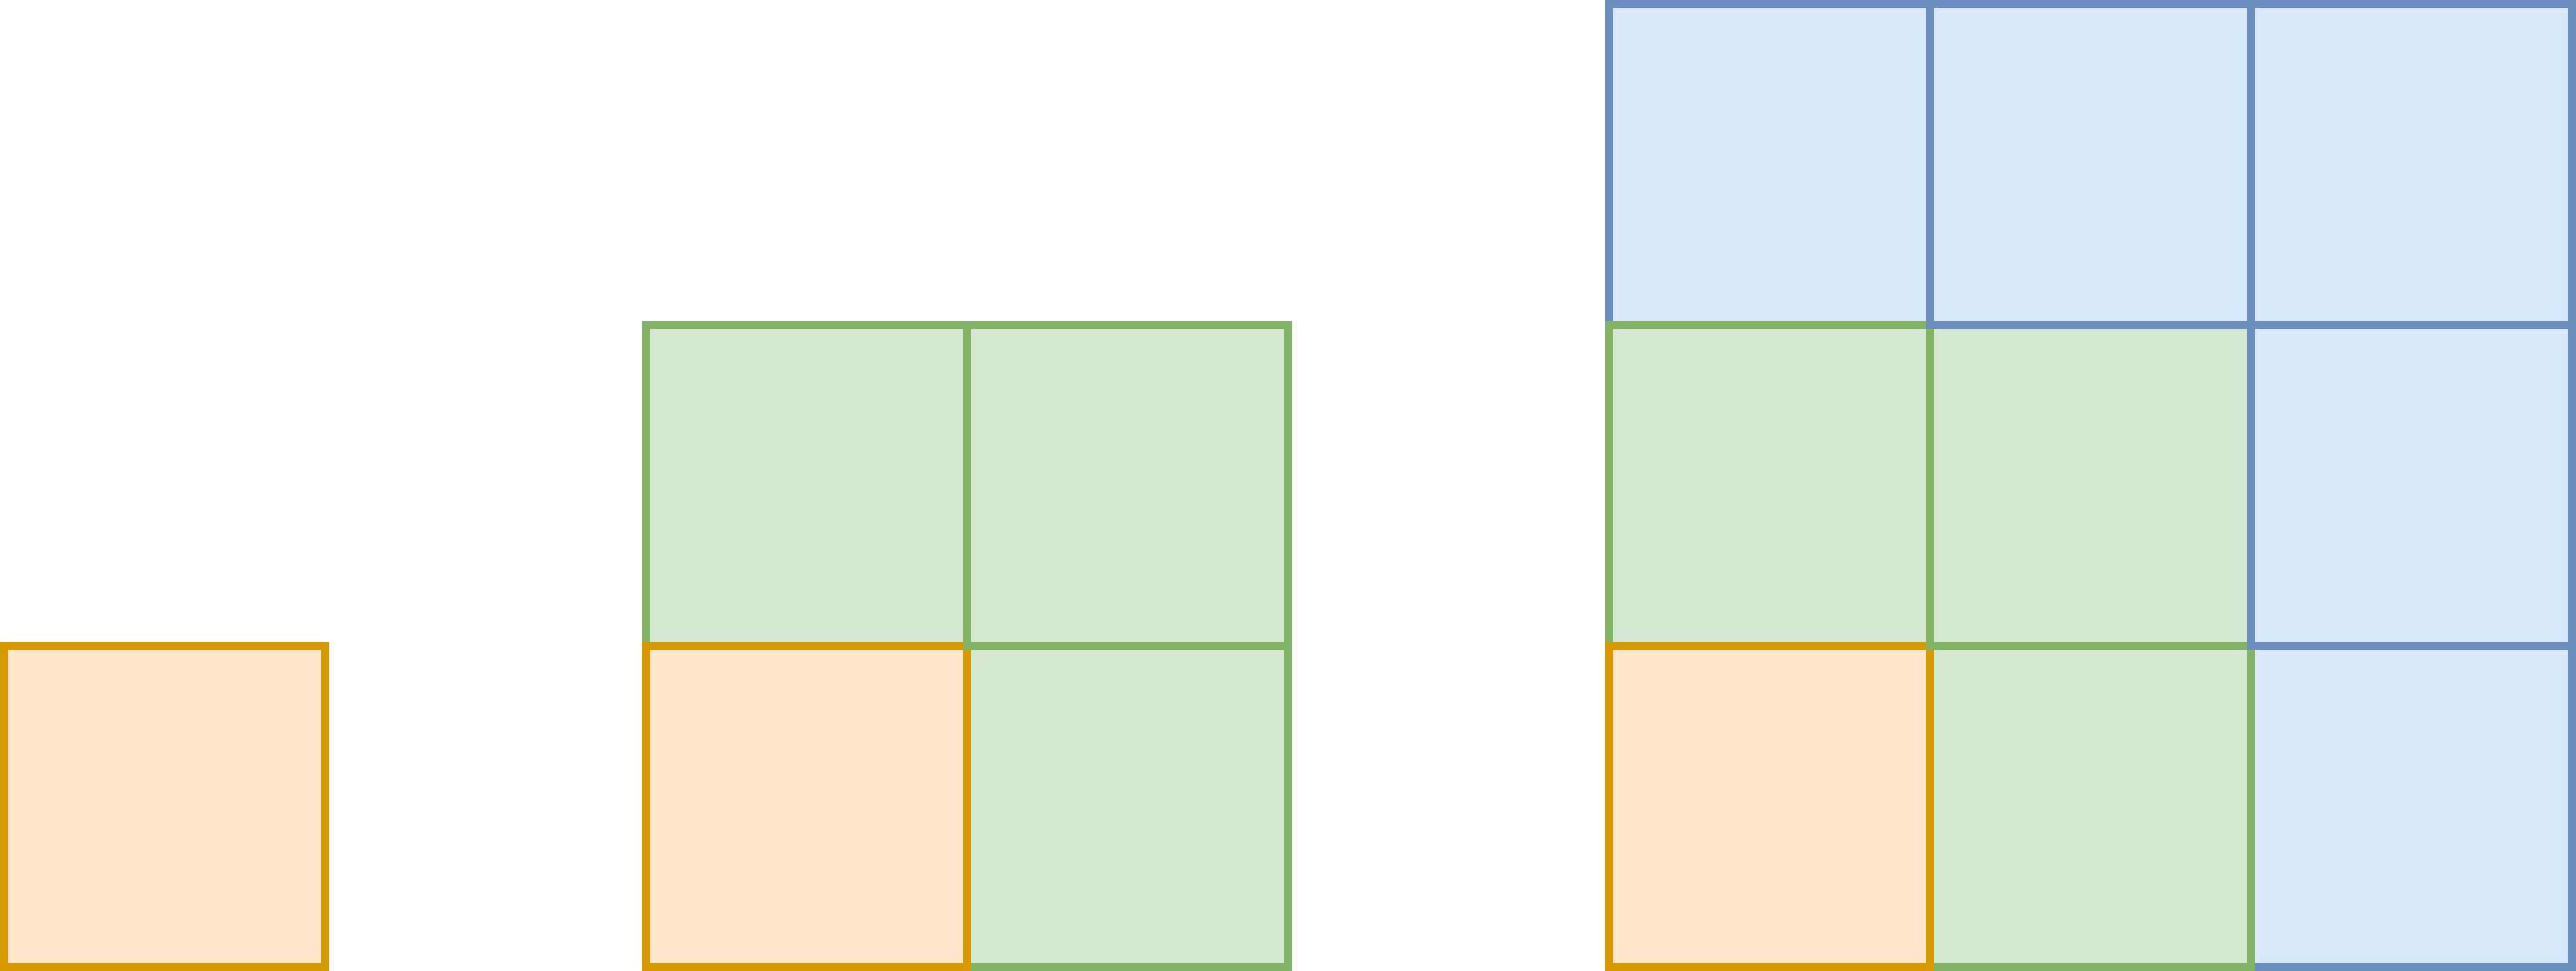
\includegraphics[width=0.5\textheight]{../figures/Summe.png}\qquad \dots
        %\caption{Idee}
        %
    \end{figure}
\end{frame}
\note[itemize]{
    \item Idee: Es werden 1, 3, 5, \ldots Felder hinzugenommen
    \item Lässt sich jeweils zu einem Quadrat zusammensetzen
    \item Mit jedem Schritt wird Kantenlänge des Quadrats um eins größer
}

\begin{frame}[fragile]{Beispiel}
    Zeigen Sie $\displaystyle\sum_{i = 0}^{n} (2i+1) = (n+1)^2,\quad\forall n \in\mathbb{N}$.
    \begin{alertblock}{Induktionsanfang (IA)}
        Zeige Aussage gilt für $n\defeq0$:\\
        \begin{align*}
                      & \sum_{i = 0}^{0} (2i+1) &  & \overset{!}{=} &  & (0+1)^2 &                  \\
            \iffspace & 2 \cdot 0 + 1           &  & \overset{!}{=} &  & 1^2     &                  \\
            \iffspace & 1                       &  & =              &  & 1       & \qquad\checkmark
        \end{align*}
    \end{alertblock}
\end{frame}

\begin{frame}[fragile]{Beispiel}
    Zeigen Sie $\displaystyle\sum_{i = 0}^{n} (2i+1) = (n+1)^2,\quad\forall n \in\mathbb{N}$.
    \begin{alertblock}{Induktionsanfang (IA)}
        Aussage gilt für $n\defeq0$, da $\displaystyle\sum_{i = 0}^{0} (2i+1) = (0+1)^2$.
    \end{alertblock}
    \begin{alertblock}{Induktionsvoraussetzung (IV)}
        Ang. Aussage gilt für (ein beliebiges aber festes) $n \in\mathbb{N}$.
    \end{alertblock}
    \begin{alertblock}{Induktionsschritt (IS)}
        Zeige Aussage gilt für alle $n+1$ unter Nutzung der (IV):\par
        $\displaystyle\sum_{i = 0}^{\alert{n+1}} (2i+1) \overset{!}{=} (\alert{(n+1)}+1)^2$
    \end{alertblock}
\end{frame}

\begin{frame}[fragile]{Beispiel}
    \small\begin{alertblock}{Induktionsschritt}
        Zeige Aussage gilt für alle $n+1$ unter Nutzung der IV:\@
        \begin{align*}
            \onslide<1->{                                 & \sum_{i = 0}^{n+1} (2i+1)                                                   &  & \overset{!}{=} &  & ((n+1)+1)^2            & } \\
            \onslide<2->{\iffspace                        & \sum_{i = 0}^{\alert<2>{n}} (2i+1) + \sum_{i = \alert<2>{n+1}}^{n+1} (2i+1) &  & \overset{!}{=} &  & (n+2)^2                & } \\
            \onslide<3->{\iffspace                        & \sum_{i = 0}^{n} (2i+1) + ( 2(n+1)+1 )                                      &  & \overset{!}{=} &  & n^2 + 2 \cdot 2n + 2^2 & } \\
            \onslide<4->{\overset{\alert<4>{IV}}\iffspace & \alert<4>{(n+1)^2} + ( 2(n+1)+1 )                                           &  & \overset{!}{=} &  & n^2+4n+4               & } \\
            \onslide<5->{\iffspace                        & n^2+2n+1^2+2n+2+1                                                           &  & \overset{!}{=} &  & n^2+4n+4               & } \\
            \onslide<6>{\iffspace                         & n^2+4n+4                                                                    &  & \alert<6>{=}   &  & n^2+4n+4               & }
        \end{align*}
    \end{alertblock}
\end{frame}

\begin{frame}[fragile]{Beispiel}
    Zeigen Sie $\displaystyle\sum_{i = 0}^{n} (2i+1) = (n+1)^2, \quad\forall n \in\mathbb{N}$.
    \begin{alertblock}{Induktionsanfang (IA)}
        Aussage gilt für $n\defeq0$, da $\displaystyle\sum_{i = 0}^{0} (2i+1) = 1^2$.
    \end{alertblock}
    \begin{alertblock}{Induktionsvoraussetzung (IV)}
        Ang. Aussage gilt für (ein beliebiges aber festes) $n \in\mathbb{N}$.
    \end{alertblock}
    \begin{alertblock}{Induktionsschritt (IS)}
        Aussage gilt für alle $n+1$ unter Nutzung der IV, da\par
        $\displaystyle\sum_{i = 0}^{n+1} (2i+1) = ((n+1)+1)^2$
    \end{alertblock}
    \alert{$\leadsto$ Aussage gilt für alle n.}\qed
\end{frame}


{\setbeamercolor{palette primary}{bg=ExColor}
\begin{frame}[fragile]{Denkpause}
    \begin{alertblock}{Aufgaben}
        Versuche dich an den folgenden Induktionsbeweisen.
    \end{alertblock}

    \metroset{block=fill}
    \begin{block}{Normal}
        $\displaystyle\sum_{i=0}^{n} i = \frac{n(n+1)}{2}, \quad \forall n \in \mathbb{N}$
    \end{block}
    \begin{block}{Schwerer}
        $\displaystyle\prod_{i=1}^{n} 4^i = 2^{n(n+1)}, \quad \forall n \in \mathbb{N}\setminus \{0\}$
    \end{block}
\end{frame}
}

%\subsubsection{Lösungen normal}
{\setbeamercolor{palette primary}{bg=ExColor}
\begin{frame}<handout:0>[fragile]{Lösungen: normale Aufgabe}
    Zu zeigen: $\displaystyle\sum_{i=0}^{n} i = \frac{n(n+1)}{2}$ gilt für alle $n \in \mathbb{N}$.
    \begin{alertblock}{Induktionsanfang (IA)}
        Aussage gilt für $n\defeq 0$, da $\displaystyle\sum_{i=0}^{0} i = 0 = \frac{0(0+1)}{2}$.
    \end{alertblock}
    \begin{alertblock}{Induktionsvoraussetzung (IV)}
        Ang. Aussage gilt für $n \in\mathbb{N}$.
    \end{alertblock}
    \begin{alertblock}{Induktionsschritt (IS)}
        Zeige Aussage gilt für alle $n+1$ unter Nutzung der IV:\par
        $\displaystyle\sum_{i=0}^{\alert{n+1}} i \overset{!}{=} \frac{(\alert{n+1})\left((\alert{n+1})+1\right)}{2}$
    \end{alertblock}
\end{frame}


\begin{frame}<handout:0>[fragile]{Lösungen: normale Aufgabe}
    \small\begin{alertblock}{Induktionsschritt}
        Zeige Aussage gilt für $n+1$ unter Nutzung der I.V.:
        \begin{align*}
            \onslide<1->{                                 & \displaystyle\sum_{i=0}^{\alert<1>{n+1}} i       &  & \overset{!}{=} &  & \frac{(\alert<1>{n+1})\left((\alert<1>{n+1})+1\right)}{2} & } \\
            \onslide<2->{\iffspace                        & \left(\displaystyle\sum_{i=0}^{n} i\right)+(n+1) &  & \overset{!}{=} &  & \frac{(n+1)(n+2)}{2}                                      & } \\
            \onslide<3->{\iffspace                        & \left(\displaystyle\sum_{i=0}^{n} i\right)+(n+1) &  & \overset{!}{=} &  & \frac{n^2+3n+2}{2}                                        & } \\
            \onslide<4->{\overset{\alert<4>{IV}}\iffspace & \alert<4>{\frac{n(n+1)}{2}}+(n+1)                &  & \overset{!}{=} &  & \frac{n^2+3n+2}{2}                                        & } \\
            \onslide<5->{\iffspace                        & \frac{n^2+n}{2}+\frac{2n+2}{2}                   &  & \overset{!}{=} &  & \frac{n^2+3n+2}{2}                                        & } \\
            \onslide<6->{\iffspace                        & \frac{n^2+3n+2}{2}                               &  & \alert{=}      &  & \frac{n^2+3n+2}{2}                                        & } \\
        \end{align*}
    \end{alertblock}
\end{frame}


\begin{frame}<handout:0>[fragile]{Lösungen: normale Aufgabe}
    Zu zeigen: $\displaystyle\sum_{i=0}^{n} i = \frac{n(n+1)}{2}$ gilt für alle $n \in \mathbb{N}$.
    \begin{alertblock}{Induktionsanfang (IA)}
        Aussage gilt für $n\defeq 0$, da $\displaystyle\sum_{i=0}^{0} i = 0 = \frac{0(0+1)}{2}$.
    \end{alertblock}
    \begin{alertblock}{Induktionsvoraussetzung (IV)}
        Ang. Aussage gilt für $n \in\mathbb{N}$.
    \end{alertblock}
    \begin{alertblock}{Induktionsschritt (IS)}
        Zeige Aussage gilt für $n+1$ unter Nutzung der IV:\par
        $\displaystyle\sum_{i=0}^{\alert{n+1}} i \overset{!}{=} \frac{(\alert{n+1})\left((\alert{n+1})+1\right)}{2}$ gilt für alle $n \in \mathbb{N}$
    \end{alertblock}
    \alert{$\leadsto$ Aussage gilt für alle $n$.}\qed
\end{frame}
}

% \begin{frame}[standout]
%   Fragen dazu?
% \end{frame}

%\subsubsection{Lösungen schwerer}
{\setbeamercolor{palette primary}{bg=ExColor}
\begin{frame}<handout:0>[fragile]{Lösungen: schwerere Aufgabe}
    Zu zeigen: $\displaystyle\prod_{i=1}^{n} 4^i = 2^{n(n+1)}$ gilt für alle $n \in \mathbb{N}\setminus \{0\}$.
    \begin{alertblock}{Induktionsanfang (IA)}
        Aussage gilt für $n\defeq 1$, da $\displaystyle\prod_{i=1}^{1} 4^i = 4^1 = 4 = 2^2 = 2^{1(1+1)}$.
    \end{alertblock}
    \begin{alertblock}{Induktionsvoraussetzung (IV)}
        Ang. Aussage gilt für $n \in\mathbb{N}\setminus \{0\}$.
    \end{alertblock}
    \begin{alertblock}{Induktionsschritt (IS)}
        Zeige Aussage gilt für $n+1$ unter Nutzung der IV:\par
        $\displaystyle\prod_{i=1}^{\alert{n+1}} 4^i \overset{!}{=} 2^{(\alert{n+1})((\alert{n+1})+1)}$
    \end{alertblock}
\end{frame}

\begin{frame}<handout:0>[fragile]{Lösungen: schwerere Aufgabe}
    \small\begin{alertblock}{Induktionsschritt}
        Zeige Aussage gilt für $n+1$ unter Nutzung der I.V.:
        \begin{align*}
            \onslide<1->{                                 & \displaystyle\prod_{i=1}^{\alert<1>{n+1}} 4^i                 &  & \overset{!}{=} &  & 2^{(\alert<1>{n+1})((\alert<1>{n+1})+1)} & } \\
            \onslide<2->{\iffspace                        & \left(\displaystyle\prod_{i=1}^{n} 4^i\right) \cdot 4^{(n+1)} &  & \overset{!}{=} &  & 2^{(n+1)(n+2)}                           & } \\
            \onslide<3->{\overset{\alert<3>{IV}}\iffspace & \alert<3>{\left(2^{n(n+1)}\right)} \cdot 4^{(n+1)}            &  & \overset{!}{=} &  & 2^{n^2+3n+2}                             & } \\
            \onslide<4->{\iffspace                        & 2^{n^2+n} \cdot 2^{2(n+1)}                                    &  & \overset{!}{=} &  & 2^{n^2+3n+2}                             & } \\
            \onslide<5->{\iffspace                        & 2^{n^2+n} \cdot 2^{2n+2}                                      &  & \overset{!}{=} &  & 2^{n^2+3n+2}                             & } \\
            \onslide<6->{\iffspace                        & 2^{(n^2+n)+(2n+2)}                                            &  & \overset{!}{=} &  & 2^{n^2+3n+2}                             & } \\
            \onslide<7->{\iffspace                        & 2^{n^2+3n+2}                                                  &  & \alert{=}      &  & 2^{n^2+3n+2}                             & }
        \end{align*}
    \end{alertblock}
\end{frame}


\begin{frame}<handout:0>[fragile]{Lösungen: schwerere Aufgabe}
    Zu zeigen: $\displaystyle\prod_{i=1}^{n} 4^i = 2^{n(n+1)}$ gilt für alle $n \in \mathbb{N}\setminus \{0\}$.
    \begin{alertblock}{Induktionsanfang (IA)}
        Aussage gilt für $n\defeq 1$, da $\displaystyle\prod_{i=1}^{1} 4^i = 4^1 = 4 = 2^2 = 2^{1(1+1)}$.
    \end{alertblock}
    \begin{alertblock}{Induktionsvoraussetzung (IV)}
        Ang. Aussage gilt für $n \in\mathbb{N}\setminus \{0\}$.
    \end{alertblock}
    \begin{alertblock}{Induktionsschritt (IS)}
        Zeige Aussage gilt für $n+1$ unter Nutzung der IV:\par
        $\displaystyle\prod_{i=1}^{\alert{n+1}} 4^i \overset{!}{=} 2^{(\alert{n+1})((\alert{n+1})+1)}$ gilt für alle $n \in \mathbb{N}\setminus \{0\}$
    \end{alertblock}
    \alert{$\leadsto$ Aussage gilt für alle $n$.}\qed
\end{frame}
}

% \begin{frame}[standout]
%   Fragen dazu?
% \end{frame}


% Copyright 2018-2022 FIUS
%
% This file is part of theo-vorkurs-folien.
%
% theo-vorkurs-folien is free software: you can redistribute it and/or modify
% it under the terms of the GNU General Public License as published by
% the Free Software Foundation, either version 3 of the License, or
% (at your option) any later version.
%
% theo-vorkurs-folien is distributed in the hope that it will be useful,
% but WITHOUT ANY WARRANTY; without even the implied warranty of
% MERCHANTABILITY or FITNESS FOR A PARTICULAR PURPOSE.  See the
% GNU General Public License for more details.
%
% You should have received a copy of the GNU General Public License
% along with theo-vorkurs-folien.  If not, see <https://www.gnu.org/licenses/>.

%Vollständige Induktion aus Tag 2
% \section{Wiederholung: Vollständige Induktion}

% \subsection{Definition}

% \begin{frame}[fragile]{Definition}
%  \begin{enumerate}
%      \item \textbf{Induktionsanfang} (Gilt die Aussage für ein $n_0$) \\
%      \item \textbf{Induktionsvoraussetzung} (wir nehmen dann an, die Aussage gilt tatsächlich)
%      \item \textbf{Induktionsschritt} (Hier zeigen wir, dass für alle $n \in \mathbb{N}$ die Aussage gilt, unter Verwendung der IV)
%  \end{enumerate}
% \end{frame}

\subsubsection{formalere Definition}
\begin{frame}{Definition nochmal formaler}
    \begin{equation*}
        (\forall n \in \mathbb{N}_{n_0}: P(n)) \iff (P(n_0) \wedge \forall n \in \mathbb{N}_{n_0}: (P(n) \implies P(n+1)))
    \end{equation*}    
\end{frame}

\begin{frame}{Definition nochmal formaler}
    \onslide<1->$(\forall n \in \mathbb{N}_{n_0}: P(n)) \iff (\alert<2>{\underbrace{P(n_0)}_{\text{IA}}}\wedge \overbrace{\alert<3>{\forall n \in \mathbb{N}_{n_0}:} (\alert<4>{\underbrace{P(n)}_{\text{IV}}} \alert<5>{\implies P(n+1)})}^{\text{IS}})$
    \begin{enumerate}
        \item<2->\alert<2>{\textbf{IA:} $n = n_0$}
        \item<3->\onslide<3->{\alert<3>{\textbf{IS:} Sei $n\in\mathbb{N}_{n_0}$ beliebig.}}
        \onslide<4->{\alert<4>{Ang. es gilt $P(n)$. \tiny{\textbf{(IV)}}}}    
        \item<5->\alert{$\leadsto$ Zeigen, dass $P(n+1)$ gilt, unter Verwendung von $P(n)$ \tiny{\textbf{(IV)}}}
    \end{enumerate}
\end{frame}

% \begin{frame}{Aufgabe zur Wiederholung}
%  Warum das ganze nur für Summen.\\
%  Angenommen $n^3-n$ ist durch 3 teilbar für alle natürlichen Zahlen.\\
%  Wie gehen wir dann hier vor?
% \end{frame}

% \begin{frame}{Aufgabe zur Wiederholung}
%  \begin{itemize}
%      \item<1->
%          Schreiben wir das ganze erst mal etwas Mathematischer.
%      \item<2->
%          $3 \mid n^3-n$, also 3 teilt $n^3-n$
%      \item<3->
%          Jetzt vollständige Induktion
%  \end{itemize}
% \end{frame}

% \begin{frame}{Vollständige Induktion}
%  \begin{enumerate}
%      \item<1->
%          \textbf{IA:} n = 1
%              \begin{equation*}
%                  3 \mid 1^3 - 1 \iff 3 \mid 1 - 1 \iff 3 \mid 0 \qquad \checkmark
%              \end{equation*}
%      \item<2->
%          % \textbf{IV:}\\
%          % Da $3 \mid n^3-n$ für 1 gilt, existiert also eine Zahl $n\in \mathbb{N}$ (beliebig aus den natürlichen Zahlen, hier 1 da wir es bereits dafür gezeigt haben), für welche die Aussage $3 \mid n^3 -n$ gilt.
%           \textbf{IS:} Sei $n \in \mathbb{N}$ beliebig. Ang., es gilt $3\mid n^3-n$ (IV)
%          \begin{align*}
%              3 \mid (n+1)^3-(n+1) &\iff 3\mid(n+1)^3 - n - 1\\
%              &\iff 3\mid n^3 + 3n^2 + 3n + 1 - n - 1\\
%              &\iff 3\mid \underbrace{n^3 - n}_{\text{Induktionsvoraussetzung}} + \underbrace{3n^2 + 3n}_{\text{vielfache von 3}} + \underbrace{1 - 1}_{= 0}\\
%              &\iff 3\mid(n^3 - n) + 3(n^2 + n)
%          \end{align*}
%      \item<3->
%      \textbf{Fazit:}\\
%          Nach Voraussetzung ist der erste Summand durch 3 teilbar, und der zweite Summand ist ein vielfaches von 3. Somit ist auch die Summe durch 3 teilbar.
%  \end{enumerate}
% \end{frame}

% \begin{frame}[fragile]{Ein Aufgabe zur Übung}
%  \begin{itemize}
%      \item Zeigen Sie, dass für alle natürlichen Zahlen $n \geq 4$ gilt: \\
%      \begin{center}
%          $n! > 2^n$\\
%      \end{center}
%  \end{itemize}
% \end{frame}

% {\setbeamercolor{palette primary}{bg=ExColor}
% \begin{frame}{Lösung}
%  \begin{enumerate}
%      \item
%          \textbf{IA:} n = 4
%          \begin{equation*}
%              4! = 4 \cdot 3 \cdot 2 \cdot 1 = 24 > 16 = 2^4
%          \end{equation*}
%      \item
%          \textbf{IV:}
%          Die Aussage $n! > 2^n$ gilt für n=4, also existiert ein $x\in \mathbb{N}$, sodass diese Aussage gilt.
%      \item
%          \textbf{IS:} Also gilt die Aussage für n+1
%          \begin{align*}
%              (n+1)! &= (n+1) \cdot n!\\
%              &\overset{\text{nach IV.}}{>} \underbrace{(n+1)}_{\text{da n min. 4}} \cdot 2^n\\
%              &\overset{(n+1)>2}{>} 2 \cdot 2^n = 2^{n+1}
%          \end{align*}
%      \item
%          \textbf{Fazit:}\\
%          Somit ist für alle $n\in \mathbb{N}$(beliebige natürliche Zahl) gezeigt, dass $n! > 2^n$ für $n \geq 4$.
%  \end{enumerate}
% \end{frame}
% }

% %An der Tafel die Lösung besprechen 


% Copyright 2018-2022 FIUS
%
% This file is part of theo-vorkurs-folien.
%
% theo-vorkurs-folien is free software: you can redistribute it and/or modify
% it under the terms of the GNU General Public License as published by
% the Free Software Foundation, either version 3 of the License, or
% (at your option) any later version.
%
% theo-vorkurs-folien is distributed in the hope that it will be useful,
% but WITHOUT ANY WARRANTY; without even the implied warranty of
% MERCHANTABILITY or FITNESS FOR A PARTICULAR PURPOSE.  See the
% GNU General Public License for more details.
%
% You should have received a copy of the GNU General Public License
% along with theo-vorkurs-folien.  If not, see <https://www.gnu.org/licenses/>.

{\setbeamercolor{palette primary}{bg=ExColor}
	\begin{frame}[fragile]{Aufgabe}
		\metroset{block=fill}
		\begin{alertblock}{Die folgende Induktion zeigt eine seltsame Aussage.}
			Ist der Beweis korrekt geführt? Was ist passiert?
		\end{alertblock}
		\metroset{block=transparent}
		Sei $A(n)\defeq$ \emph{In einer Herde aus $n$ Telefonen haben alle die selbe Farbe.}\\
		Zu zeigen: $A(n)$ gilt für alle $n \in \mathbb{N} \setminus \{0\} $.
		\begin{alertblock}{Induktionsanfang (IA)}
			$A(1)$: Aussage gilt für $n\defeq 1$, da ein Telefon nur eine Farbe haben kann.
		\end{alertblock}
		\begin{alertblock}{Induktionsvoraussetzung (IV)}
			Ang. $A(n)$ gilt für $n\geq1$.
		\end{alertblock}
		\begin{alertblock}{Induktionsschritt (IS)}
			Zeige Aussage gilt für alle $n+1$ unter Nutzung der IV:\\
			D.h. wir zeigen $A(n+1)=$ \emph{In einer Herde aus $n+1$ Telefonen haben alle die selbe Farbe.}
		\end{alertblock}
	\end{frame}
	\begin{frame}[fragile]{Aufgabe}
		\footnotesize{
			\begin{alertblock}{Induktionsschritt (IS)}
				Wir betrachten eine Herde aus $n+1$ Telefonen:
				\[\underbrace{\text{\Telefon}\text{\Telefon}\text{\Telefon}\text{\Telefon}\text{\Telefon}\dots\text{\Telefon}\text{\Telefon}}_{n+1}\]
				Wir sondern ein Telefon aus und betrachten den Rest. Nach I.V. haben diese alle die selbe Farbe.
				\[\underbrace{\alert{\text{\Telefon}\text{\Telefon}\text{\Telefon}\text{\Telefon}\text{\Telefon}\dots\text{\Telefon}}}_{n}\text{\Telefon}\]
				Jetzt sondern wir ein anderes Telefon aus.
				\[\alert{\text{\Telefon}}\underbrace{\alert{\text{\Telefon}\text{\Telefon}\text{\Telefon}\text{\Telefon}\dots\text{\Telefon}}\text{\Telefon}}_{n}\]
				Die übrigen $n$ Telefone haben nach I.V. wieder die selbe Farbe.
				\[\underbrace{\alert{\text{\Telefon}\text{\Telefon}\text{\Telefon}\text{\Telefon}\text{\Telefon}\dots\text{\Telefon}\text{\Telefon}}}_{n+1}\]
				Also haben alle $n+1$ Telefone die selbe Farbe.
				$\leadsto$ $A(n)$ gilt für alle $n$.
			\end{alertblock}
		}
	\end{frame}
}

{\setbeamercolor{palette primary}{bg=ExColor}
	\begin{frame}<handout:0>[fragile]{Lösungen}
		\small{
			\metroset{block=fill}
			\begin{block}{Das Problem}
				Für $A(n+1)$ wird angenommen, dass beide Herden der $n$ Telefone mindestens ein gemeinsames Element haben. 
				Sie teilen dann die Farbe dieses Elements. 

				Das Problem ist, dass $A(1) \Rightarrow A(2)$ nicht zwangsweise erfüllt sein muss! Somit können wir keine weiteren Folgerungen über $A(n+1)$ mit $n \geq 2$ machen.
				
				\begin{figure}
				\resizebox{.4\textwidth}{!}{
					\centering%
					\begin{subfigure}{0.3\textwidth}
						\centering%
						
\includegraphics[height=0.5in]{../figures/telephoneGreen.png}
					\end{subfigure}
					$\qquad$
					\begin{subfigure}{0.3\textwidth}
						\centering%
						
\includegraphics[height=0.5in]{../figures/telephoneWhite.png}
					\end{subfigure}
					}
					\caption{Beide Telefone erfüllen jeweils $A(1)$, zusammen aber nicht $A(2)$}
				\end{figure}

				Denn es gibt ein überlappendes Element erst ab $n+1=3$ Telefonen:
				\[
					A(3):\alert{\rlap{$\overbrace{\phantom{\text{\Telefon\Telefon}}}^{A(2)}$}\text{\Telefon}\underbrace{\text{\Telefon\Telefon}}_{A(2)}}
					\leadsto A(4):\alert{\rlap{$\overbrace{\phantom{\text{\Telefon\Telefon\Telefon}}}^{A(3)}$}\text{\Telefon}\underbrace{\text{\Telefon\Telefon\Telefon}}_{A(3)}}
					\leadsto \dots \leadsto A(n+1): \alert{\rlap{$\overbrace{\phantom{\text{\Telefon\Telefon} ... \text{\Telefon}}}^{A(n)}$}\text{\Telefon}\underbrace{\text{\Telefon} ... \text{\Telefon\Telefon}}_{A(n)}}
				\]

			\end{block}
		}
	\end{frame}
	\note{
		Einordnung der Grafiken:
		\begin{itemize}
			\item In der ersten Grafik wird gezeigt, dass das Argument für $A(k)$ mit $k \geq 3$ funktioniert falls man $A(2)$ annimmt. 
			\item Die zweite Grafik zeigt nun aber auf, dass man nicht einfach $A(2)$ annehmen kann!
		\end{itemize}

		\alert{Optional:} Wieso ist das aus formaler Sicht ein Problem?

		Betrachtet man die Definition von Induktion (angewandt auf unseren Beweis)
		\begin{align*}
			\underbrace{(\forall n \in \mathbb{N}_1: A(n))}_{(*)} \iff (A(1) \wedge \forall n \in \mathbb{N}_1: \underbrace{(A(n) \implies A(n+1))}_{(**)}),
		\end{align*}
		so sieht man, dass $(**)$ für $n=1$ nicht funktioniert (siehe zweite Grafik). Damit ist $(*)$ falsch!
	}
}



\metroset{sectionpage=none,subsectionpage=progressbar}

\section{Prädikatenlogik}
\begin{frame}[fragile]{7-Segment Anzeigen}
	\metroset{block=fill}
	\begin{block}{Können Zahlen zeigen}
		\begin{center}
			\sevensegnum[size=15mm]{2}%
			\hspace{1em}
			\sevensegnum[size=15mm]{0}%
			\hspace{1em}
			\sevensegnum[size=15mm]{2}%
			\hspace{1em}
			\sevensegnum[size=15mm]{5}%
		\end{center}
	\end{block}
	\pause
	\begin{block}{Zeigen manchmal wirres Zeugs}
		\begin{center}
			\sevenseg[size=15mm]{0,0,0,1,0,0,0,}%
			\hspace{1em}
			\sevenseg[size=15mm]{0,1,0,0,1,0,0,}%
			\hspace{1em}
			\sevenseg[size=15mm]{1,1,0,1,1,1,1,}%
			\hspace{1em}
			\sevenseg[size=15mm]{1,0,1,1,0,0,0,}%
		\end{center}
	\end{block}
\end{frame}

\begin{frame}{\only<2->{\xout}{Der Checker} \only<2->{Das Prädikat}}
	Wir brauchen einen \textit{Checker}:
	\Huge
	\begin{center}
		$
			\only<1,2>{P_{\text{Zahl}}\left(\sevensegnum{6}\right)}
			\only<3->{P_{\text{Zahl}}\left(\sevenseg{{1,0,1,1,0,0,0,}}\right)}
		$
	\end{center}
	\normalsize
	% todo
	\only<1>{Wenn wir in diesen \textit{Checker} (genannt Prädikat) eine Anzeige einsetzen, haben wir eine logische Aussage}
	\only<2-3>{
		\begin{tikzpicture}[overlay]
			\node[] at (5,.8) (base) {};
			\node[] at (2, -.4) (wahr) {
				\only<2>{\alert}{Wahr}, wenn eine Zahl zu sehen ist
			};
			\draw[->] (base) to (wahr);
			\only<3>{\node[] at (8, -.4) (wahr) {
					\alert{Falsch}, wenn keine Zahl zu sehen ist
				};
				\draw[->] (base) to (wahr);
			}
		\end{tikzpicture}
	}
\end{frame}

{\setbeamercolor{palette primary}{bg=ExColor}
\begin{frame}{Denkpause}
	Sind die folgenden Aussagen wahr oder falsch
	\metroset{block=fill}
	\begin{block}{Normal}
		\begin{itemize}
			\item $A_1$: $P_{\text{Zahl}}\left(\sevensegnum[]{7}\right)$ \only<2->{\hspace{1cm}wahr}
			\item $A_2$: $P_{\text{Zahl}}\left(\sevenseg[]{0,1,0,0,1,0,1}\right)$ \only<3->{\hspace{1cm}falsch}
			\item $A_3$: $P_{\text{Zahl}}\left(\sevensegnum[]{4}\right)$ \only<4->{\hspace{1cm}wahr}
			\item $A_4$: $P_{\text{Zahl}}\left(\sevenseg[]{1,0,1,0,1,0,1}\right)$ \only<5>{\hspace{1cm}falsch}
		\end{itemize}
	\end{block}
\end{frame}
}

\begin{frame}{Zurück zu unserem Beispiel}
	Wie reparieren wir die Anzeige?
	\begin{center}
		\sevenseg[size=15mm]{0,0,0,1,0,0,0,}
		\hspace{1em}
		\sevenseg[size=15mm]{0,1,0,0,1,0,0,}
		\hspace{1em}
		\sevenseg[size=15mm]{1,1,0,1,1,1,1,}
		\hspace{1em}
		\sevenseg[size=15mm]{1,0,1,1,0,0,0,}
	\end{center}
\end{frame}

\begin{frame}{Funktionen}
	Wir brauchen eine Funktion, die Segmente einschaltet
	\Large
	\begin{center}
		$
			f_{\text{On}}\left(
			\sevenseg[size=10mm]{1,0,0,1,0,0,1,},
			\sevenseg[size=10mm]{0,1,1,0,1,1,0,}
			\right) =
			\sevenseg[size=10mm]{1,1,1,1,1,1,1,}
		$
	\end{center}
\end{frame}


\begin{frame}{Reicht das?}
	\begin{itemize}
		\item<1-> $f_{\text{On}}\left(\sevenseg{{0,0,0,1,0,0,0,}}, \only<1>{\hspace{1em}}\only{\sevenseg{{1,1,0,0,1,0,1,}}}<2->\right) = \sevensegnum{2}$
		\item<3-> $f_{\text{On}}\left(\sevenseg{{0,1,0,0,1,0,0,}}, \only<3>{\hspace{1em}}\only{\sevenseg{{1,0,1,1,0,1,0,}}}<4->\right) = \sevensegnum{0}$
		\item<5-> $f_{\text{On}}\left(\sevenseg{{1,1,0,1,1,1,1,}}, \only<5>{\hspace{1em}}\only{\textcolor{red}{X }}<6->\right) = \sevensegnum{2}$
		\item<7-> $f_{\text{On}}\left(\sevenseg{{1,0,1,1,0,0,0,}}, \only<7>{\hspace{1em}}\only{\sevenseg{{0,0,0,0,0,1,1,}}}<8->\right) = \sevensegnum{5}$
	\end{itemize}
\end{frame}


\begin{frame}{Mehr Funktionen}
	\Large
	\begin{center}
		$
			f_{\text{Off}}\left(
			\sevenseg[size=10mm]{{1,1,1,1,1,1,1,}},
			\sevenseg[size=10mm]{{0,1,1,1,1,1,0,}}
			\right) =
			\sevenseg[size=10mm]{{1,0,0,0,0,0,1,}}
		$
	\end{center}
	\normalsize
\end{frame}

\begin{frame}{Mehr Funktionen}
	\Large
	\begin{center}
		$
			f_{\text{Off}}\left(
			\sevenseg[size=10mm]{1,1,1,1,1,1,1,},
			\sevenseg[size=10mm]{1,1,1,1,1,1,0,}
			\right) =
			\sevenseg[size=10mm]{0,0,0,0,0,0,1,}
		$
	\end{center}
	\normalsize
\end{frame}


\begin{frame}{Beides Zusammen}
	Kombiniert mit unserem \alert{Prädikt}:
	\Large
	\begin{center}
		$
			P_{\text{Zahl}}\left(f_{\text{On}}\left(
			\sevenseg[size=10mm]{1,0,0,0,0,0,0,},
			\sevenseg[size=10mm]{0,1,1,0,0,0,0,}
			\right)\right)
		$
	\end{center}
	\normalsize
	\pause
	Diese Aussage ist wahr
	\par
	\pause
	Allgemeiner:
	$U =\left\{\sevensegnum[]{0},\sevenseg{{0,1,1,0,1,1,1,}},\sevensegnum[]{2},\sevenseg{{0,1,1,0,0,0,0,}},\sevensegnum[]{4},\sevenseg{{0,0,0,0,0,0,0,}},\sevenseg{{0,1,1,1,1,1,0,}},\sevensegnum[]{7},\sevensegnum[]{8},\sevenseg{{0,0,1,0,1,1,1,}}, \dots \right\}$
	$$
		\forall X\in U:\exists Y \in U: P_{Zahl}(f_{On}(X,Y))
	$$
	$U =\left\{\randsevenseg,\randsevenseg,\randsevenseg,\randsevenseg,\randsevenseg,\randsevenseg,\randsevenseg,\randsevenseg, \dots \right\}$
	$$
		\forall X\in U:\exists Y \in U: P_{Zahl}(f_{On}(X,Y))
	$$
	Das \alert{Universum} ist die Menge aller Werte, die in unsere Formel eingesetzt werden können.
\end{frame}

{\setbeamercolor{palette primary}{bg=ExColor}
\begin{frame}{Denkpause}
	Finde Anzeigen für die Variablen $X, Y$, für die die Aussage stimmt
	\metroset{block=fill}
	\begin{block}{Normal}
		\begin{itemize}
			\item $P_{\text{Zahl}}\left(f_{\text{On}}\left(\sevenseg{{0,0,0,0,0,0,0,}}, X_1\right)\right)$
			\item $P_{\text{Zahl}}\left(f_{\text{Off}}\left(X_2, Y_2\right)\right)$
			\item $P_{\text{Zahl}}\left(f_{\text{Off}}\left(X_3, \sevenseg{{0,0,0,0,1,1,0,0,}}\right)\right) \land P_{\text{Zahl}}\left(f_{\text{On}}\left(X_3, \sevenseg{{1,0,0,1,0,0,0,}}\right)\right)$
			\item $\lnot P_{\text{Zahl}}\left(f_{\text{On}}\left(f_{\text{On}}\left(\sevenseg{{0,0,0,0,0,0,0,}}, X_4\right), \sevenseg{{1,1,1,1,0,0,1,}}\right)\right)$
		\end{itemize}
	\end{block}
	Beweise ob die folgenden Aussagen wahr oder falsch sind
	\metroset{block=fill}
	\begin{block}{Etwas schwerer}
		\begin{itemize}
			\item $A_5$: $\forall X : P_{\text{Zahl}}\left(f_{\text{On}}\left(X, \sevenseg{{1,1,1,1,1,1,1,1,}}\right)\right)$
			\item $A_6$: $\forall X \exists Y : P_{\text{Zahl}}\left(X\right) \implies \lnot P_{\text{Zahl}}\left(f_{\text{On}}\left(X,Y\right)\right)$
		\end{itemize}
	\end{block}
\end{frame}
}

{\setbeamercolor{palette primary}{bg=ExColor}
\begin{frame}<handout:0>{Lösungen}
	\textit{Für 1-4 je Beispiele, es gibt weitere Lösungen}
	\begin{itemize}[<+- | alert@+>]
		\item $X_1 \in \left\{\sevensegnum{0},\sevensegnum{1},\sevensegnum{2},\dots\right\}$
		\item $X_2 = \sevensegnum{8}, y_2 = \sevenseg{{0,0,0,0,0,0,1,}}$ oder $X_2 = \sevensegnum{4}, y_2 = \sevenseg{{1,0,0,1,1,1,0,0,}}$
		\item $X_3 = \sevenseg{{0,1,1,0,1,1,0,}}$
		\item $X_4 = \sevenseg{{0,0,0,0,1,0,0,}}$
		\item \textit{wahr}\\
		      Beweis: Zu einer beliebigen Anzeige alle Segmente einzuschalten sorgt dafür, dass alle Segmente eingeschaltet sind,\\
		      Alle Segmente eingeschaltet ist eine gültige Zahl ($8$)
		\item \textit{falsch}\\
		      Gegenbeispiel: $\sevensegnum{8}$ (Beweis wie oben)
	\end{itemize}
\end{frame}
}

\begin{frame}{Rätselaufgabe}
	Fällt euch ein Prädikat $P_{?}$ ein, für das die folgende Aussage wahr ist:
	\Large
	$$\forall X \in U \setminus \{\sevensegnum[]{8},\sevensegnum[]{0}\}: P_{\only<1>{?}\only<2->{\alert{\leq 6}}}(X)$$
	\pause
	\normalsize
	Passende Prädikate:
	\begin{itemize}
		\item $P_{\leq 6}$ : wahr, wenn mindestens 6 Segmente eingeschaltet sind
		      \pause
		\item $P_{\text{rahmen-an}}$ : wahr, wenn alle äußeren Segmente eingeschaltet sind
		\item $P_{\text{wahr}}$ immer wahr
		\item ...
	\end{itemize}
	\pause
	Nicht passsende Prädikate:
	\begin{itemize}
		\item $P_{\text{mitte-an}}$ : wahr, wenn das horizontale mittlere Segment eingeschaltet is
		\item $P_{\text{falsch}}$ : nie wahr
		\item ...
	\end{itemize}
\end{frame}

\begin{frame}{Prädikatssymbole}
	\begin{itemize}[<+- | alert@+>]
		\item Prädikatenlogische Formeln haben ihre Preädikate und Funktionen nicht unbedingt festgelegt
		\item Sie können auch aus Prädikatenymbolen und Formelsymbolen bestehen
		\item Unsere Aufgabe ist dann sie zu interpretieren
	\end{itemize}
\end{frame}

\begin{frame}{Definitionen}
	\metroset{block=fill}
	\begin{block}{Prädikate}
		\begin{itemize}
			\item $P_{Zahl}(X):$ Die Anzeige $X$ zeigt eine Zahl.
			\item $P_<7(X):$ Die Anzeige $X$ hat maximal 6 leuchtende Segmente.
			      \pause
			\item $P_=(X,Y):$ Die Anzeigen $X$ und $Y$ sind gleich.
			\item $P_>(X,Y):$ Die Anzeige $X$ hat mehr leuchtende Segmente als die Anzeige $Y$.
		\end{itemize}
	\end{block}
	\begin{block}{Funktionen}
		\begin{itemize}
			\item $f_{ON}(X,Y):$ Schalte alle Segmente an, welche in $X$ oder $Y$ an sind.
			\item $f_{OFF}(X,Y):$ Scahlte alle Segmente an, welche in $X$ and sind aber nicht in $Y$.
			\item $f_{INV}(X):$ Schalte alle Segmente an, welche in $X$ aus sind.
			\item $f_{COUNT}(X,Y):$ Zeige die Zahl an, die angibt wie viele Segmente in $X$ an sind.
		\end{itemize}
	\end{block}
	\begin{block}{Das Universum}
		$U =\left\{\randsevenseg,\randsevenseg,\randsevenseg,\randsevenseg,\randsevenseg,\randsevenseg,\randsevenseg,\randsevenseg, \dots \right\}$
	\end{block}
\end{frame}

\begin{frame}{Eine Interpretation erstellen}
	Nun wollen wir für die folgende Prädikantelogoische Formel eine Interpretation erstellen:
	$$
		\forall X\exists Y: P_0(f_0(X),f_1(Y))
	$$
	\pause
	\begin{columns}
		\begin{column}{.45\textwidth}
			\begin{itemize}[<+- | alert@+>]
				\item $I(P_0) = P_=$
				\item $I(f_0) = f_{ZAHL}$
				\item $I(f_1) = f_{INV}$
			\end{itemize}
		\end{column}
		\begin{column}{.45\textwidth}
			\only<5>{
				\begin{itemize}
					\item $I(P_0) = P_=$
					\item $I(f_0) = f_{ZAHL}$
					\item $I(f_1) = f_{ZAHL}$
				\end{itemize}
			}
		\end{column}
	\end{columns}
\end{frame}

{\setbeamercolor{palette primary}{bg=ExColor}
\begin{frame}{Denkpause}
	Finde Interpretationen, für die die Aussagen stimmen
	\metroset{block=fill}
	\begin{block}{Normal}
		\begin{itemize}
			\item $\overline{P_0(f_0(X,Y), f_1(Y,X))}$
		\end{itemize}
	\end{block}
\end{frame}

\begin{frame}<handout:0>{Lösungen}
	\textit{Für 1-4 je Beispiele, es gibt weitere Lösungen}
	\begin{itemize}[<+- | alert@+>]
		\item TODO
	\end{itemize}
\end{frame}
}

\begin{frame}{Ganz Generisch}
	\begin{itemize}[<+->]
		\item Eigentlich haben wir kein Universum, keine  Prädikate und keine Funktionen vorgegeben
		\item Gegeben ist nur eine Prädikatenlogische Formel
		\item Wir müssen bestimmen ob diese irgendwie erfüllbar ist
	\end{itemize}
\end{frame}

\begin{frame}{Beispiel}
	\begin{center}
		\begin{tikzpicture}[overlay]

			\only<3,6, 11>{
				\node[] (a) at (-2cm, 0){\textcolor{green}{JA}};
				\draw[->] (a) to (-2.4cm, -1cm);
			}
			\only<5,7,8, 10>{
				\node[] (a) at (-2cm, 0){\textcolor{red}{NEIN}};
				\draw[->] (a) to (-2.4cm, -1cm);
			}

			\only<5,7,8,10,11>{
				\node[] (b) at (0,0) {\textcolor{green}{JA}};
				\draw[->] (b) to (0, -1cm);
			}
			\only<3,6>{
				\node[] (b) at (0,0) {\textcolor{red}{NEIN}};
				\draw[->] (b) to (0, -1cm);
			}

			\only<5,7,8,10,11>{
				\node[] (c) at (2cm, 0) {\textcolor{green}{JA}};
				\draw[->] (c) to (2.4cm, -1cm);
			}
			\only<3,6>{
				\node[] (c) at (2cm, 0) {\textcolor{red}{NEIN}};
				\draw[->] (c) to (2.4cm, -1cm);
			}
		\end{tikzpicture}
	\end{center}

	$$
		(\forall X \exists Y: P(X,Y)) \wedge (\forall X: \overline{P(X,X)}) \wedge (\exists X \overline{P(Y,X)})
	$$

	\begin{center}
		\begin{tikzpicture}[
				base/.style={draw, circle, minimum size = .3cm}
			]
			\only<4->{\node[base] (n0) at (0,0){0};}
			\only<6>{\draw[thick,->] (n0.90) arc (0:270:3mm);}

			\only<7->{\node[base, below left = of n0] (n1) {1};}

			\only<9->{\node[base, below right = of n0] (n2) {2};}


			\only<8,10,11>{\draw[thick,->] (n0) to (n1);}
			\only<10,11>{\draw[thick,->, bend right] (n1) to (n0);}
			\only<11>{\draw[thick,->, bend right] (n2) to (n0);}
		\end{tikzpicture}

		%

		\only<1-3>{Können wir die Formel mit dem Universum $U= \emptyset$ erfüllen?}
		\only<4-6>{Was ist mit dem Universum, das ein Element hat. Nennen wir das Element mal $0$}
		\only<7-8>{Lasst es uns mal mit $U= \{0,1\}$ probieren}
		\only<9->{Lasst es uns mal mit $U= \{0,1,2\}$ probieren}
	\end{center}

\end{frame}

\begin{frame}{Formal aufschreiben}
	\alert{Achtung:} Man muss das Ergebnis formal aufschreiben!

	\begin{align*}
		U             & = \{0,1,2\}                            \\
		I(P)          & = \{(0,1), (1,0), (2,1)\}              \\
		\only<3>{I(f) & = \{0\mapsto1, 1\mapsto2, 2\mapsto0\}}
	\end{align*}

	\begin{tikzpicture}[overlay]
		\only<2>{
			\node[] (a) at (7cm,3cm) {Das Universum};
			\node[] (b) at (5,.6) {alle Kombinationen für die das Prädikat zu einer wahren Aussage wird};
			\draw[->] (a) to (5.62cm, 2.4cm);
			\draw[->] (b) to (5.3cm, 1.5cm);
		}
		\only{
			\node[] (b) at (5,-.4) {Wenn man eine Funktion hat, wird diese so angegeben};
			\draw[->] (b) to (5.3cm, .8cm);
		}<3>
	\end{tikzpicture}


\end{frame}

{\setbeamercolor{palette primary}{bg=ExColor}
\begin{frame}{Denkpause}
	Finde Interpretationen, für die die Aussagen stimmen
	\metroset{block=fill}
	\begin{block}{Normal}
		\begin{itemize}
			\item TODO
		\end{itemize}
	\end{block}
\end{frame}

\begin{frame}<handout:0>{Lösungen}
	\textit{Für 1-4 je Beispiele, es gibt weitere Lösungen}
	\begin{itemize}[<+- | alert@+>]
		\item TODO
	\end{itemize}

\end{frame}
}
\subsection{Generisch}

\begin{frame}{Ganz Generisch}
    \begin{itemize}[<+->]
        \item Eigentlich haben wir kein Universum, keine Prädikate und keine Funktionen vorgegeben
        \item Gegeben ist nur eine Prädikatenlogische Formel
        \item Wir müssen bestimmen ob diese irgendwie erfüllbar ist
    \end{itemize}
\end{frame}

\begin{frame}{Beispiel}
    \note{Dieses Beispiel erweitert das Universum immer um ein Element und geht ein paar Möglichkeiten durch das Prädikat anzuwenden.
        Ein Pfeil von Knoten $X$ auf $Y$ im Graphen bedeutet, dass das $P(X, Y)$ wahr ist, ein fehlender Pfeil, dasss es falsch ist.
        \par
        Dieses Beispiel wurde aus der Ergänzung für Theo II 2018 von Carlos Carmino übernommen
        https://fmi.uni-stuttgart.de/ti/teaching/s18/eti2/ (Termin 1)
    }
    \begin{center}
        \begin{tikzpicture}[overlay]
            \only<1>{\node[] at (0cm,-5cm){\tiny Dieses Beispiel wurde aus der Ergänzung für Theo II 2018 von Carlos Carmino übernommen
                    \url{https://fmi.uni-stuttgart.de/ti/teaching/s18/eti2/}}};

            \only<4,8>{
                \node[] (a) at (-2cm, 0){\textcolor{green}{JA}};
                \draw[->] (a) to (-2.4cm, -1cm);
            }
            \only<3,5,6,7>{
                \node[] (a) at (-2cm, 0){\textcolor{red}{NEIN}};
                \draw[->] (a) to (-2.4cm, -1cm);
            }

            \only<3,5,6,7,8>{
                \node[] (b) at (0,0) {\textcolor{green}{JA}};
                \draw[->] (b) to (0, -1cm);
            }
            \only<4>{
                \node[] (b) at (0,0) {\textcolor{red}{NEIN}};
                \draw[->] (b) to (0, -1cm);
            }

            \only<3,5,6,7,8>{
                \node[] (c) at (2cm, 0) {\textcolor{green}{JA}};
                \draw[->] (c) to (2.4cm, -1cm);
            }
            \only<4>{
                \node[] (c) at (2cm, 0) {\textcolor{red}{NEIN}};
                \draw[->] (c) to (2.4cm, -1cm);
            }
        \end{tikzpicture}
    \end{center}

    $$
        (\forall X \exists Y: P(X,Y)) \wedge (\forall X: \lnot P(X,X)) \wedge (\exists X \forall Y : \lnot P(Y,X))
    $$

    \begin{center}
        \begin{tikzpicture}[
                base/.style={draw, circle, minimum size = .3cm}
            ]
            \only<2->{\node[base] (n0) at (0,0){0};}
            \only<4>{\draw[thick,->] (n0.90) arc (0:270:3mm);}

            \only<5->{\node[base, below left = of n0] (n1) {1};}

            \only<7->{\node[base, below right = of n0] (n2) {2};}


            \only<6,7,8>{\draw[thick,->] (n0) to (n1);}
            \only<7,8>{\draw[thick,->, bend right] (n1) to (n0);}
            \only<8>{\draw[thick,->, bend right] (n2) to (n0);}
        \end{tikzpicture}

        %

        \only<1>{$U= \emptyset$ müssen wir nicht testen, da das Universum nicht leer sein darf}
        \only<2-4>{Was ist mit dem Universum, das ein Element hat. Nennen wir das Element mal $0$}
        \only<5-6>{Lasst es uns mal mit $U= \{0,1\}$ probieren}
        \only<7->{Lasst es uns mal mit $U= \{0,1,2\}$ probieren}
    \end{center}

\end{frame}

\begin{frame}{Formal aufschreiben}
    \alert{Achtung:} Wir müssen das Ergebnis formal aufschreiben!

    \begin{align*}
        U                                   & = \{0,1,2\}                                                      \\
        I(P)                                & = \{(0,1), (1,0), (2,1)\}                                        \\
        \onslide<3->{\textcolor{gray}{I(f)} & = \textcolor{gray}{\{0 \mapsto 1, 1 \mapsto 2, 2 \mapsto 0\} } } \\
        \onslide<4->{I(a)                   & = 0}
    \end{align*}

    \begin{tikzpicture}[overlay]
        \only<2>{
            \node[] (a) at (7cm,3.5cm) {Das Universum};
            \node[] (b) at (5,1.1) {alle Kombinationen für die das Prädikat zu einer wahren Aussage wird};
            \draw[->] (a) to (5.62cm, 2.9cm);
            \draw[->] (b) to (5.3cm, 2cm);
        }
        \only{
            \node[] (b) at (5,-.4) {Wenn man eine Funktion hat, wird diese so angegeben};
            \node[] at (5,-.9) {(Haben wir im Beispiel nicht)};
            \draw[->] (b) to (5.3cm, 1.5cm);
        }<3>
        \only{
            \node[] (b) at (5,-.4) {Wenn man eine Konstante hat, wird sie so angegeben};
            \node[] at (5,-.9) {(Haben wir im Beispiel nicht)};
            \draw[->] (b) to (4.3cm, .8cm);
        }<4>
    \end{tikzpicture}


\end{frame}

{\setbeamercolor{palette primary}{bg=ExColor}
\begin{frame}{Denkpause}
    Finde Interpretationen, für die die Aussagen stimmen
    \metroset{block=fill}
    \begin{block}{Normal}
        \begin{itemize}
            \item $\forall x: {P_0(x,f(x))}$
            \item $\forall x\ \forall y : P_1(x,y)\land \forall x : \lnot P_1(a_2,x)$ mit $a_2$ Konstante
            \item $\forall x : \left(P_2(x,f(x))\land P_3(f(x),x)\right)$ mit $U=\mathbb{N}$ %Lösung: f: Nachfolge, P: <, Q: >
            \item $\forall x\ \forall y\ \forall z : \left(\left(P_4(x,y) \land P_4(y,z)\right)\implies P_4(x,z)\right) \land \forall x\ \forall y : \left(\lnot P_4(x,y) \lor \lnot P_4(y,x)\right) \land \forall y\ P_4(a_4, y)$ mit $a_4$ Konstante
        \end{itemize}
    \end{block}
    \begin{block}{Schwer}
        \begin{itemize}
            \item $\left(\forall X\ \exists\ Y \forall\ Z \in U\setminus\{y\} : P_5(X,Y)\land\lnot P_5(X,Y)\right) \land \left(\forall X,Y\ \exists Z_0,\dots,Z_n : P_5(X,Z_0) \land \left(\bigwedge_{i=0}^{n-1} P_5(Z_i,Z_{i+1})\right) \land P_5(Z_n,Y)\right)$
        \end{itemize}
    \end{block}
\end{frame}

\begin{frame}<handout:0>{Lösungen}
    \textit{Für 1-4 je Beispiele, es gibt weitere Lösungen}
    \begin{itemize}[<+- | alert@+>]
        \item TODO
    \end{itemize}

\end{frame}

\begin{frame}{Zum Knobeln}
    \small
    \metroset{block=fill}
    \begin{block}{}
        \begin{multicols}{2}
            \begin{itemize}
                \item $F_1 = \forall X \exists Y: P_0(X,Y)$
                \item $F_2 = \forall X: \overline{P_0(X,X)}$
                \item $F_3 = \exists Y \forall X: \overline{P_0(X,Y)}$
                \item $F_4 = \forall X: \overline{P_0(X,f(x))}$
                \item {\scriptsize$F_5 = \forall X \forall Y: (P_0(X,f(Y)) \implies P_0(Y,X))$}
                \item $F_6 = P(a, f(f(a)))$
                \item $F_7 = \forall X (\exists Y: P_0(Y,X)\implies P_1(X))$
                \item $F_8 = \overline{P_1(f(f(b)))}$
                \item $F_9 = P(f(c),c)$
            \end{itemize}
        \end{multicols}
        Gib eine Interpretation für $F = \bigwedge_{i=1}^9 F_i$ an
    \end{block}
\end{frame}
}

\metroset{sectionpage=progressbar,subsectionpage=none}

\section{Modulare Arithmetik}
\begin{frame}{Motivation}
    \begin{center}
        \begin{center}
            \Large
            Rechnen mit unendlich vielen Zahlen ist hart
        \end{center}
        \pause
        \vspace{1cm}

        \begin{tikzpicture}[x=.5cm,y=1cm]

            % The number line with arrows on both ends
            \draw[<->] (-6,0) -- (6,0);

            % Infinity hints
            \node[above] at (-6,0) {$-\infty$};
            \node[above] at (6,0) {$+\infty$};

            % Tick marks (loop)
            \foreach \x in {-5,-4,...,5}
            \draw (\x,0.1) -- (\x,-0.1);

            % Labels for nonzero ticks (loop)
            \foreach \x in {-5,-4,...,-1,1,2,...,5}
            \node[below] at (\x,-0.1) {\small \x};

            % Thicker tick and label for zero
            \draw[thick] (0,0.15) -- (0,-0.15);
            \node[below] at (0,-0.15) {\small 0};

        \end{tikzpicture}
    \end{center}
\end{frame}

\begin{frame}{Motivation}
    \begin{center}
        \begin{center}
            \Large
            Wir können einfach nur mit den Zahlen $0$ bis $5$ rechnen
        \end{center}
        \pause
        \vspace{1cm}

        \begin{tikzpicture}[x=.5cm,y=1cm]

            % The number line with arrows on both ends
            \draw[-] (-6,0) -- (6,0);

            % Tick marks (loop)
            \foreach \x in {0,...,5}
            \draw (\x,0.1) -- (\x,-0.1);

            % Labels for nonzero ticks (loop)
            \foreach \x in {1,2,...,5}
            \node[below] at (\x,-0.1) {\small \x};

            % Thicker tick and label for zero
            \draw[thick] (0,0.15) -- (0,-0.15);
            \node[below] at (0,-0.15) {\small 0};

        \end{tikzpicture}
    \end{center}
    \pause
    \begin{center}
        \Large
        Was ist jetzt $3+4$?
    \end{center}
\end{frame}

\begin{frame}[fragile]{Motivation}
    \begin{center}
        \vspace{1cm}

        \begin{tikzpicture}[x=1cm,y=1cm]

            % Draw the circle
            \draw (0,0) circle (2);

            % Place the numbers 0 to 5 equally spaced
            \foreach \i in {0,...,5} {
                    \node[font=\small] at ({-60*(\i-1)}:2.2) (\i){\i}; % labels slightly outside
                    \draw[-] ({60*\i}:1.9) to ({60*\i}:2.1);
                }

            \pause
            \draw[-, in = -180, out = -120] (3) to (4);
            \draw[-, in = -240, out = -180] (4) to (5);
            \draw[-, in = -300, out = -240] (5) to (0);
            \draw[->, in = -360, out = -300] (0) to (1);



        \end{tikzpicture}
    \end{center}
\end{frame}

\begin{frame}[fragile]{Wiederholung: Modulo}
    \begin{center}
        \Large
        $$
            3+4 \equiv 1 \mod 6
        $$

        \pause
        Das bedeutet so viel wie:

        $$
            (3+4)\% 6 = 1 \% 6
        $$
    \end{center}
\end{frame}


\begin{frame}[fragile]{Restklassenring}
    \begin{itemize}
        \item Wir nennen so einen begrenzten Zahlenraum \alert{Restklassenring}
        \item Die mathematische Schreibweise für einen Restklassenring mit $m$ Zahlen aus $\mathbb{Z}$ ist:
              $$
                  \mathbb Z / m\mathbb Z
              $$
    \end{itemize}
\end{frame}

{\setbeamercolor{palette primary}{bg=ExColor}
\begin{frame}[fragile]{Denkpause}
    \footnotesize
    \begin{alertblock}{Aufgaben}
    \end{alertblock}
    \metroset{block=fill}
    \begin{block}{löst die folgenden Rechenaufgaben im $\mathbb Z/12\mathbb Z$}
        \begin{multicols}{3}
            \begin{itemize}
                \item $10 + 2$
                \item $3\cdot4-1$
                \item $(2-4)2$
            \end{itemize}
        \end{multicols}
    \end{block}
    \begin{block}{löst die folgenden Rechenaufgaben im $\mathbb Z/7\mathbb Z$}
        \begin{multicols}{3}
            \begin{itemize}
                \item $5 + 1$
                \item $3\cdot4-1$
                \item $(2-4)2+5$
                \item $5^2$
                \item $0\cdot4$
                \item $5!$
            \end{itemize}
        \end{multicols}
    \end{block}
    \begin{block}{Was ist $m$?}
        \begin{multicols}{3}
            \begin{itemize}
                \item $4 \equiv 6 \mod m$
                \item $3 \equiv 9 \mod m$
                \item $4 \equiv 11 \mod m$
            \end{itemize}
        \end{multicols}
    \end{block}
\end{frame}

\begin{frame}<handout:0>{Lösungen}
    \begin{itemize}[<+- | alert@+>]
        \item $10+2 \equiv 0 \mod 12$
        \item $3\cdot 4-1 \equiv 11 \mod 12$
        \item
              \begin{align*}
                  (2-4)2 & \equiv x \mod 12 \\
                  (-2)2  & \equiv x \mod 12 \\
                  -4     & \equiv x \mod 12 \\
                  12-4   & =8
              \end{align*}

              oder
              \begin{align*}
                  (2-4)2 & \equiv x \mod 12 \\
                  (-2)2  & \equiv x \mod 12 \\
                  (10)2  & \equiv x \mod 12 \\
                  20     & \equiv x \mod 12 \\
                  20-12  & = 8
              \end{align*}
    \end{itemize}
\end{frame}

\begin{frame}<handout:0>{Lösungen}
    \begin{itemize}[<+- | alert@+>]
        \item $5 + 1      \equiv 6 \mod 7$
        \item $3\cdot4-1  \equiv 4 \mod 7$
        \item $(2-4)2+5   \equiv 1 \mod 7$
        \item $5^2        \equiv 4 \mod 7$
        \item $0\cdot4    \equiv 0 \mod 7$
        \item $5!         \equiv 1 \mod 7$
    \end{itemize}
\end{frame}

\begin{frame}<handout:0>{Lösungen}
    \begin{itemize}[<+- | alert@+>]
        \item $4 \equiv 6 \mod m$

              $m \in \{1,2\}$
        \item $3 \equiv 9 \mod m$

              $m \in \{1,3\}$
        \item $4 \equiv 11 \mod m$

              $m \in \{1,7\}$
    \end{itemize}
\end{frame}
}

\begin{frame}{Wofür brauchen wir das?}
    \begin{outline}
        \1 Computer sind nicht unendlich groß
        \2 Variablen verbrauchen eine fixe Menge Platz
        \2 Was machen wenn die Zahl zu groß wird für diesen Platz?
        \2 Z.B. der unsigned Integer ist im $\mathbb Z / 2^{64}\mathbb Z$
        \pause
        \1 Hashing / Checksums
        \2 Wie stelle ich sicher ob eine Datei die Datei ist, die ich haben will?
        \pause
        \1 Verschlüsselung
        \2 Moderne Kryptographie verwendet die modulare Arithmetik

    \end{outline}
\end{frame}

{\setbeamercolor{palette primary}{bg=ExColor}
\begin{frame}[fragile]{Knobelaufgabe}
    \footnotesize
    \metroset{block=fill}
    \begin{block}{Finde eine Zahl $n \in \mathbb N$ für die alle folgenden Eigenschaften gelten:}
        \begin{multicols}{2}
            \begin{itemize}
                \item $n \equiv m \mod 2$
                \item $m \in \{2x | x \in \mathbb N\}$
                \item $n \equiv k \mod 17$
                \item  $\exists x: m-x < 0 \wedge m\cdot x < 100$
            \end{itemize}
        \end{multicols}
    \end{block}

\end{frame}

}

\section{Wiederholung}
\input{../parts/wdh_slides/induktion.tex}
\begin{frame}[fragile]{Das können wir jetzt beantworten}
	\begin{alertblock}{Prädikatenlogik}
		\begin{itemize}
			\item todo
		\end{itemize}
	\end{alertblock}
\end{frame}
\begin{frame}{Motivation}
    \begin{center}
        \begin{center}
            \Large
            Rechnen mit unendlich vielen Zahlen ist hart
        \end{center}
        \pause
        \vspace{1cm}

        \begin{tikzpicture}[x=.5cm,y=1cm]

            % The number line with arrows on both ends
            \draw[<->] (-6,0) -- (6,0);

            % Infinity hints
            \node[above] at (-6,0) {$-\infty$};
            \node[above] at (6,0) {$+\infty$};

            % Tick marks (loop)
            \foreach \x in {-5,-4,...,5}
            \draw (\x,0.1) -- (\x,-0.1);

            % Labels for nonzero ticks (loop)
            \foreach \x in {-5,-4,...,-1,1,2,...,5}
            \node[below] at (\x,-0.1) {\small \x};

            % Thicker tick and label for zero
            \draw[thick] (0,0.15) -- (0,-0.15);
            \node[below] at (0,-0.15) {\small 0};

        \end{tikzpicture}
    \end{center}
\end{frame}

\begin{frame}{Motivation}
    \begin{center}
        \begin{center}
            \Large
            Wir können einfach nur mit den Zahlen $0$ bis $5$ rechnen
        \end{center}
        \pause
        \vspace{1cm}

        \begin{tikzpicture}[x=.5cm,y=1cm]

            % The number line with arrows on both ends
            \draw[-] (-6,0) -- (6,0);

            % Tick marks (loop)
            \foreach \x in {0,...,5}
            \draw (\x,0.1) -- (\x,-0.1);

            % Labels for nonzero ticks (loop)
            \foreach \x in {1,2,...,5}
            \node[below] at (\x,-0.1) {\small \x};

            % Thicker tick and label for zero
            \draw[thick] (0,0.15) -- (0,-0.15);
            \node[below] at (0,-0.15) {\small 0};

        \end{tikzpicture}
    \end{center}
    \pause
    \begin{center}
        \Large
        Was ist jetzt $3+4$?
    \end{center}
\end{frame}

\begin{frame}[fragile]{Motivation}
    \begin{center}
        \vspace{1cm}

        \begin{tikzpicture}[x=1cm,y=1cm]

            % Draw the circle
            \draw (0,0) circle (2);

            % Place the numbers 0 to 5 equally spaced
            \foreach \i in {0,...,5} {
                    \node[font=\small] at ({-60*(\i-1)}:2.2) (\i){\i}; % labels slightly outside
                    \draw[-] ({60*\i}:1.9) to ({60*\i}:2.1);
                }

            \pause
            \draw[-, in = -180, out = -120] (3) to (4);
            \draw[-, in = -240, out = -180] (4) to (5);
            \draw[-, in = -300, out = -240] (5) to (0);
            \draw[->, in = -360, out = -300] (0) to (1);



        \end{tikzpicture}
    \end{center}
\end{frame}

\begin{frame}[fragile]{Wiederholung: Modulo}
    \begin{center}
        \Large
        $$
            3+4 \equiv 1 \mod 6
        $$

        \pause
        Das bedeutet so viel wie:

        $$
            (3+4)\% 6 = 1 \% 6
        $$
    \end{center}
\end{frame}


\begin{frame}[fragile]{Restklassenring}
    \begin{itemize}
        \item Wir nennen so einen begrenzten Zahlenraum \alert{Restklassenring}
        \item Die mathematische Schreibweise für einen Restklassenring mit $m$ Zahlen aus $\mathbb{Z}$ ist:
              $$
                  \mathbb Z / m\mathbb Z
              $$
    \end{itemize}
\end{frame}

{\setbeamercolor{palette primary}{bg=ExColor}
\begin{frame}[fragile]{Denkpause}
    \footnotesize
    \begin{alertblock}{Aufgaben}
    \end{alertblock}
    \metroset{block=fill}
    \begin{block}{löst die folgenden Rechenaufgaben im $\mathbb Z/12\mathbb Z$}
        \begin{multicols}{3}
            \begin{itemize}
                \item $10 + 2$
                \item $3\cdot4-1$
                \item $(2-4)2$
            \end{itemize}
        \end{multicols}
    \end{block}
    \begin{block}{löst die folgenden Rechenaufgaben im $\mathbb Z/7\mathbb Z$}
        \begin{multicols}{3}
            \begin{itemize}
                \item $5 + 1$
                \item $3\cdot4-1$
                \item $(2-4)2+5$
                \item $5^2$
                \item $0\cdot4$
                \item $5!$
            \end{itemize}
        \end{multicols}
    \end{block}
    \begin{block}{Was ist $m$?}
        \begin{multicols}{3}
            \begin{itemize}
                \item $4 \equiv 6 \mod m$
                \item $3 \equiv 9 \mod m$
                \item $4 \equiv 11 \mod m$
            \end{itemize}
        \end{multicols}
    \end{block}
\end{frame}

\begin{frame}<handout:0>{Lösungen}
    \begin{itemize}[<+- | alert@+>]
        \item $10+2 \equiv 0 \mod 12$
        \item $3\cdot 4-1 \equiv 11 \mod 12$
        \item
              \begin{align*}
                  (2-4)2 & \equiv x \mod 12 \\
                  (-2)2  & \equiv x \mod 12 \\
                  -4     & \equiv x \mod 12 \\
                  12-4   & =8
              \end{align*}

              oder
              \begin{align*}
                  (2-4)2 & \equiv x \mod 12 \\
                  (-2)2  & \equiv x \mod 12 \\
                  (10)2  & \equiv x \mod 12 \\
                  20     & \equiv x \mod 12 \\
                  20-12  & = 8
              \end{align*}
    \end{itemize}
\end{frame}

\begin{frame}<handout:0>{Lösungen}
    \begin{itemize}[<+- | alert@+>]
        \item $5 + 1      \equiv 6 \mod 7$
        \item $3\cdot4-1  \equiv 4 \mod 7$
        \item $(2-4)2+5   \equiv 1 \mod 7$
        \item $5^2        \equiv 4 \mod 7$
        \item $0\cdot4    \equiv 0 \mod 7$
        \item $5!         \equiv 1 \mod 7$
    \end{itemize}
\end{frame}

\begin{frame}<handout:0>{Lösungen}
    \begin{itemize}[<+- | alert@+>]
        \item $4 \equiv 6 \mod m$

              $m \in \{1,2\}$
        \item $3 \equiv 9 \mod m$

              $m \in \{1,3\}$
        \item $4 \equiv 11 \mod m$

              $m \in \{1,7\}$
    \end{itemize}
\end{frame}
}

\begin{frame}{Wofür brauchen wir das?}
    \begin{outline}
        \1 Computer sind nicht unendlich groß
        \2 Variablen verbrauchen eine fixe Menge Platz
        \2 Was machen wenn die Zahl zu groß wird für diesen Platz?
        \2 Z.B. der unsigned Integer ist im $\mathbb Z / 2^{64}\mathbb Z$
        \pause
        \1 Hashing / Checksums
        \2 Wie stelle ich sicher ob eine Datei die Datei ist, die ich haben will?
        \pause
        \1 Verschlüsselung
        \2 Moderne Kryptographie verwendet die modulare Arithmetik

    \end{outline}
\end{frame}

{\setbeamercolor{palette primary}{bg=ExColor}
\begin{frame}[fragile]{Knobelaufgabe}
    \footnotesize
    \metroset{block=fill}
    \begin{block}{Finde eine Zahl $n \in \mathbb N$ für die alle folgenden Eigenschaften gelten:}
        \begin{multicols}{2}
            \begin{itemize}
                \item $n \equiv m \mod 2$
                \item $m \in \{2x | x \in \mathbb N\}$
                \item $n \equiv k \mod 17$
                \item  $\exists x: m-x < 0 \wedge m\cdot x < 100$
            \end{itemize}
        \end{multicols}
    \end{block}

\end{frame}

}

\Center{Noch Fragen?}

\section{Wiederholungsaufgaben}
\begin{frame}[fragile]{Das können wir jetzt beantworten}
	\begin{alertblock}{Mengen, Sprachen, Elemente}
		\begin{itemize}
			\item Was ist eine Menge?
			\item Was ist eine Sprache?
			\item Was sind Elemente einer Sprache/Menge?
		\end{itemize}
	\end{alertblock}
\end{frame}

\begin{frame}[fragile]{Das können wir jetzt beantworten}
	\begin{alertblock}{Operationen auf Mengen}
		\begin{itemize}
			\item Wie funktionieren Vereinigung, Schnitt und Komplement?
			\item Wie bilde ich die Vereinigung oder Schnittmenge zweier Mengen?
			\item Wie bilde ich das Komplement einer Menge?
			\item Wie kann ich Sprachen formal beschreiben?
			\item Hantieren mit verschiedenen seltsamen Mengen und den Verknüpfungen
		\end{itemize}
	\end{alertblock}
\end{frame}
\begin{frame}[fragile]{Was ist Aussagenlogik?}
    \begin{alertblock}{Aussagen}
    \begin{itemize}
        \item Paris ist die Hauptstadt von Frankreich
        \item Mäuse jagen Elefanten
        \item $5 \in \mathbb{N}$
        \item 5 = 8
        \item $u \in \{u, v, w\}$
    \end{itemize}
    \end{alertblock}
    Eine Aussage A ist entweder \textbf{wahr} oder \textbf{falsch}.
\end{frame}

\begin{frame}[fragile]{Was ist Aussagenlogik?}
    \begin{alertblock}{Das sind keine Aussagen}
    \begin{itemize}
        \item Macht theoretische Informatik Spaß?
        \item Geh dein Zimmer aufräumen!
        \item Wie viele Tiere wohnen in der Uni?
        \item $(x+y)^2+1$
        \item \{a,b,c\}
        \item ...
    \end{itemize}
    \end{alertblock}
    Diesen Sätzen können wir keinen eindeutigen Wahrheitswert \textbf{wahr} oder \textbf{falsch} zuordnen.
\end{frame}

\begin{frame}[fragile]{Was ist Aussagenlogik?}
    \begin{alertblock}{Wozu brauchen wir das?}
    \begin{itemize}
        \item Wir untersuchen, wie wir Aussagen verknüpfen können.
        \item Damit ziehen wir formale Schlüsse und führen Beweise.
    \end{itemize}
    \end{alertblock}
\end{frame}

\begin{frame}[fragile]{Logische Operationen}
Wir können Aussagen verändern oder durch Operationen zu neuen Aussagen verbinden.
\begin{itemize}
    \item A: Fred möchte Schokolade.
    \item B: Fred möchte Gummibärchen.
\end{itemize}
\metroset{block=fill}
\begin{alertblock}{Grundoperationen}
\begin{itemize}
    \item<1-> \textbf{Und}: A \alert<1>{$\wedge$} B $\leadsto$ Fred möchte Schokolade \alert<1>{und} Gummibärchen.\\
    \only<1>{\emph{Analog}: M: $M_1 \cap M_2$, Jedes Element aus M liegt in $M_1$ \textbf{und} in $M_2$}
    \item<2-> \textbf{Oder}: A \alert<2>{$\vee$} B $\leadsto$ Fred möchte Schokolade \alert<2>{oder} Gummibärchen.\\
    \only<2>{\emph{Anmerkung}: Inklusives \glqq oder\grqq, kein \glqq entweder oder\grqq \\
    Das heißt, es können auch beide Aussagen wahr sein.\\}
	\only<2>{\emph{Analog}: M: $M_1 \cup M_2$, Jedes Element aus M liegt in $M_1$ \textbf{oder} in $M_2$}
    \item<3> \textbf{Nicht}: \alert<3>{$\neg$}A $\leadsto$ Fred möchte \alert<3>{keine} Schokolade.\\
    \only<3>{\emph{Analog}: M: $\overline{M_1}$, Jedes Element aus M liegt \textbf{nicht} in $M_1$}
\end{itemize}
\end{alertblock}
\end{frame}


\begin{frame}{Überblick: Mengenoperationen}
	
	Auf \alert{Mengen} A, B lassen sich verschiedene Mengenoperationen ausführen.
	
	\metroset{block=fill}
	\begin{exampleblock}{Mengenoperationen}
		\begin{itemize}
			\item Schnitt: $A \cap B$
			\item Vereinigung: $A \cup B$
			\item Komplement: $\overline{A}$
		\end{itemize}
	\end{exampleblock}
\end{frame}

\begin{frame}{Überblick: Logische Operationen}
	
	Auf \alert{Aussagen} A, B lassen sich verschiedene logische Operationen ausführen.
	
	\metroset{block=fill}
	\begin{exampleblock}{Logische Operationen}
		\begin{itemize}
			\item Logisches Und: $A \wedge B$
			\item Logisches Oder: $A \vee B$
			\item Logisches Nicht: $\neg A$
		\end{itemize}
	\end{exampleblock}
\end{frame}

{\setbeamercolor{palette primary}{bg=ExColor}
	\begin{frame}{Logische Operationen vs. Mengenoperationen}
		\alert{Mengenoperationen und logische Operationen dürfen nicht verwechselt werden.}
		\begin{table}[]
			\begin{tabular}{l l}
				A: $5 \in \mathbb{N}$ & B: Es regnet\\
				C: \{$w \mid |w|=2$ \} \ & D: \{a,b,c,x,y\}\\
			\end{tabular}
		\end{table}
		\metroset{block=fill}
		\metroset{block=fill}
		\begin{block}{Welche dieser Verknüpfungen sind zulässig?}
			\begin{itemize}
				\item $L_1: A \wedge B$
				\item $L_2: A \vee C$
				\item $L_3: C \cap D$
				\item $L_4: A \wedge B \cup C$
			\end{itemize}
		\end{block}
	\end{frame}
}

{\setbeamercolor{palette primary}{bg=ExColor}
	\begin{frame}[fragile]{Logische Operationen vs. Mengenoperationen}
		\begin{itemize}[<+- | alert@+>]
			\item $L_1$: Zulässig
			\item $L_2$: Nicht zulässig
			\item $L_3$: Zulässig
			\item $L_4$: Nicht zulässig
		\end{itemize}
	\end{frame}
}



\begin{frame}{Logische Operationen: Implikation}
\begin{alertblock}{A$\implies$B}
\begin{itemize}
    \item \glqq Wenn A wahr ist, dann muss auch B wahr sein.\grqq
    \item kurz: \glqq\textbf{Wenn} A, \textbf{dann} B.\grqq
    \item Wenn A falsch ist können wir keine Aussage über B treffen.
    \item A$\implies$B ist dieselbe Aussage wie $\neg A \vee B$
\end{itemize}
\end{alertblock}
\end{frame}

\begin{frame}{Logische Operationen: Äquivalenz}
\begin{alertblock}{A$\iff$B}
\begin{itemize}
    \item \glqq A ist wahr, \textbf{genau dann wenn} B wahr ist.\grqq
    \item kurz: \glqq A gdw. B\grqq
    \item A und B müssen den selben Wahrheitswert haben.
    \item A$\iff$B ist dieselbe Aussage wie $(A \implies B) \wedge (B \implies A)$
\end{itemize}
\end{alertblock}
\end{frame}

{\setbeamercolor{palette primary}{bg=ExColor}
\begin{frame}[fragile]{Denkpause}
    \begin{alertblock}{Aufgaben}
      Berechne den Wahrheitswert folgender Aussagen. 
    \end{alertblock}
    \metroset{block=fill}
    \begin{block}{Normal}
    \begin{itemize}
        \item $A_1$: $5 \in \mathbb{N} \wedge a \in \{a, b, c\}$
        \item $A_2$: $0 \in \mathbb{N} \vee a \in \{a, b, c, d\}$
        \item $A_3$: $A_1 \iff A_2$
    \end{itemize}
    \end{block}
    \begin{block}{Etwas Schwerer}
    \begin{itemize}
        \item $A_4$: $(\emptyset=\emptyset^{*}) \implies (a \in \emptyset)$
        \item $A_5$: $(a \notin \emptyset) \implies (\emptyset = \emptyset^{*})$
        \item $A_6$: $A_4 \iff A_5$
        \item $A_7$: $(7 \in \{1, 2, 7, 9\}) \cap (2 = 7-5)$
        \item $A_8$: Wenn mein Auto fliegt, dann hast du auch ein fliegendes Auto.
    \end{itemize}
    \end{block}
\end{frame}
}

% {\setbeamercolor{palette primary}{bg=ExColor}
% \begin{frame}[fragile]{Denkpause}
%     \begin{alertblock}{Aufgaben}
%       Löse folgende Zusatzaufgabe. 
%     \end{alertblock}
%     \metroset{block=fill}
%     \begin{block}{Zusatz}
%     \begin{itemize}
%         \item $A_8$: Gegeben zwei Aussagen A, B.\\
%         Formuliere die Aussage $A \iff B$ nur unter Verwendung der Junktoren $\wedge, \vee, \neg$
%     \end{itemize}
%     \end{block}
% \end{frame}
% }

{\setbeamercolor{palette primary}{bg=ExColor}
\begin{frame}{Lösungen}
  \begin{itemize}[<+- | alert@+>]
        \item 
            $A_1$: wahr
        \item
            $A_2$: wahr
        \item
            $A_3$: wahr
        \item
            $A_4$: wahr 
        \item
            $A_5$: falsch
       	\item
       		$A_6$: falsch
        \item
            $A_7$: Das ist keine Aussage, da der Schnitt($\cap$) verwendet wurde um zwei Aussagen miteinander zu verknüpfen
       	\item
       		$A_8$: wahr
    \end{itemize}
\end{frame}
}

\begin{frame}[standout]
    Murmelpause
\end{frame}

% {\setbeamercolor{palette primary}{bg=ExColor}
% \begin{frame}{Lösungen}
%     \metroset{block=fill}
%     \begin{block}{Zusatz}
%     \begin{itemize}
%         \item $A_8$: Gegeben zwei Aussagen A, B.\\
%         Formuliere die Aussage $A \iff B$ nur unter Verwendung der Junktoren $\wedge, \vee, \neg$
%     \end{itemize}
%     \end{block}
%   \begin{alertblock}{Lösung}
%         \begin{itemize}[<+- | alert@+>]
%             \item Äquivalenz bedeutet intuitiv: Beide wahr oder beide falsch
%             \item $A_8$: $(A \wedge B) \vee (\neg A \wedge \neg B)$
%         \end{itemize}
%   \end{alertblock}
% \end{frame}
% }




\begin{frame}{Anwendung der Implikation}
    Wir haben zwei Aussagen $A$ und $B$. Wir nehmen nun an, $A$ sei wahr. Wenn wir zeigen, dass dann auch $B$ wahr ist, wissen wir, dass $A \implies B$ gilt.
\metroset{block=fill}
\begin{exampleblock}{Beispiel}
\begin{enumerate}
    \item<1-> Wir wollen zeigen, dass für eine ganze Zahl $x$ \\
    die Implikation $3 = x - 2 \implies x = 5$ gilt.
    \item<2-> Wir nehmen an, dass die linke Aussage wahr ist\dots
    \item<3-> \dots und zeigen, dass dann die rechte Aussage gilt.
    \item<4-> $(3 = x - 2) \implies (3 + 2 = x) \implies (5 = x) \implies (x = 5)$
    \item<5-> Also folgt die rechte Aussage aus der linken
    \item<6-> Somit gilt die Implikation \qed\;
\end{enumerate}
\end{exampleblock}
\end{frame}

% {\setbeamercolor{palette primary}{bg=ExColor}
% \begin{frame}{Denkpause}
%     \begin{alertblock}{Aufgaben}
%       Welche der folgenden Schlüsse sind richtig? 
%     \end{alertblock}
%     \metroset{block=fill}
%     \begin{block}{Normal bis Schwer}
%     \begin{itemize}
%         \item $S_1$: Lukas ist im Vorkurs oder schläft noch. Im Vorkurs ist er nicht. Also schläft er noch.
%         \item $S_2$: Wenn Anne nicht rennt, bekommt sie die Bahn nicht. Sie bekommt die Bahn. Also ist sie gerannt.
%         \item $S_3$: Wenn Tobi nicht lernt, besteht er nicht. Tobi hat gelernt. Also besteht er.
%     \end{itemize}
%     \end{block}
% \end{frame}
% }

% {\setbeamercolor{palette primary}{bg=ExColor}
% \begin{frame}{Lösungen}
%   \begin{itemize}[<+- | alert@+>]
%         \item 
%             $S_1$: Richtig.
%         \item
%             $S_2$: Richtig. Begründung: Die zweite Aussage ist die Kontraposition der ersten Aussage. Wie gezeigt wurde, ist die Kontraposition einer Aussage wahr gdw. die Aussage selbst wahr ist.
%         \item
%             $S_3$: Falsch. Beispiel: Tobi lernt, und besteht trotzdem nicht. \Frowny
%     \end{itemize}
% \end{frame}
% }


\begin{frame}[fragile]{Das können wir jetzt beantworten}
	\begin{alertblock}{Mengen, Sprachen, Elemente}
		\begin{itemize}
			\item Was ist eine Menge?
			\item Was ist eine Sprache?
			\item Was sind Elemente einer Sprache/Menge?
		\end{itemize}
	\end{alertblock}
\end{frame}

\begin{frame}[fragile]{Das können wir jetzt beantworten}
	\begin{alertblock}{Operationen auf Mengen}
		\begin{itemize}
			\item Wie funktionieren Vereinigung, Schnitt und Komplement?
			\item Wie bilde ich die Vereinigung oder Schnittmenge zweier Mengen?
			\item Wie bilde ich das Komplement einer Menge?
			\item Wie kann ich Sprachen formal beschreiben?
			\item Hantieren mit verschiedenen seltsamen Mengen und den Verknüpfungen
		\end{itemize}
	\end{alertblock}
\end{frame}
\begin{frame}[fragile]{Glossar - Aussagenlogik}
    \small
    \begin{tabular}{p{0.33\textwidth} p{0.2\textwidth} p{0.45\textwidth}}
        \toprule
        Abk.                     & Bedeutung                                       & Was?!                                                              \\
        \midrule
        $A\land B$               & A \textit{und} B                                & A und B müssen wahr sein, damit die Gesamtaussage wahr ist         \\
        $A\lor B$                & A \textit{oder} B                               & Es müssen mindestend A, B oder beide wahr sein                     \\
        $\lnot A$                & \textit{nicht} A                                & A muss falsch sein, damit $\lnot A$ wahr ist                       \\
        $B \implies B$           & A ist notwendig für B                           & A muss wahr sein, wenn B wahr ist                                  \\
        $A \implies B$           & A ist hinreichend für / impliziert B            & B muss wahr sein, wenn A wahr ist                                  \\
        $A \iff B$               & notwendig und hinreichend                       & genau dann, wenn                                                   \\
        $\forall x \in M : A(x)$ & Für alle $x$ aus $M$ gilt $A(x)$                & Die Aussage $A$ muss für alle Elemente der Menge $M$ wahr sein     \\
        $\exists x \in M : A(x)$ & Es existiert ein $x$ in $M$ für das $A(x)$ gilt & Die Aussage $A(x)$ muss für mind. 1 (oder mehr) Elemente wahr sein \\
        \bottomrule
    \end{tabular}
\end{frame}
\begin{frame}[fragile]{Glossar \textemdash\ Quantoren}
    \small
    \begin{tabular}{p{0.33\textwidth} p{0.2\textwidth} p{0.45\textwidth}}
        \toprule
        Abk.                         & Bedeutung                                        & Was?!                                                              \\
        \midrule
        $\forall x \in M : A(x)$     & Für alle $x$ aus $M$ gilt $A(x)$                 & Die Aussage $A$ muss für alle Elemente der Menge $M$ wahr sein     \\
        $\exists x \in M : A(x)$     & Es existiert ein $x$ in $M$ für das $A(x)$ gilt  & Die Aussage $A(x)$ muss für mind. 1 (oder mehr) Elemente wahr sein \\
        $\forall x,y \in M : A(x,y)$ & Für alle $x$ \textit{und} alle $y$ gilt $A(x,y)$ & Äquivalent zu $\forall x \forall y : A(x,y)$                       \\
        \bottomrule
    \end{tabular}
\end{frame}
% Copyright 2018, 2019, 2020, 2021 FIUS
%
% This file is part of theo-vorkurs-folien.
%
% theo-vorkurs-folien is free software: you can redistribute it and/or modify
% it under the terms of the GNU General Public License as published by
% the Free Software Foundation, either version 3 of the License, or
% (at your option) any later version.
%
% theo-vorkurs-folien is distributed in the hope that it will be useful,
% but WITHOUT ANY WARRANTY; without even the implied warranty of
% MERCHANTABILITY or FITNESS FOR A PARTICULAR PURPOSE.  See the
% GNU General Public License for more details.
%
% You should have received a copy of the GNU General Public License
% along with theo-vorkurs-folien.  If not, see <https://www.gnu.org/licenses/>.

{\setbeamercolor{palette primary}{bg=ExColor}
\begin{frame}[fragile]{Beweise}
	\begin{alertblock}{Aufgaben}
		Versuche dich an folgenden Beweisen:
	\end{alertblock}
	\metroset{block=fill}
	\begin{block}{Normal}
		Sei $L = \{a^nb^n \mid n \in \mathbb{N}\}$, dann gilt:
		\begin{align*}
			\forall w \in \{a, b\}^*: \left(w \in L \implies |w| \text{ ist gerade}\right)
		\end{align*}
	\end{block}
	\metroset{block=fill}
	\begin{block}{Wer noch nicht genug hat...}
		\begin{align*}
			\forall x \in \mathbb{Z}: x \equiv 0 \pmod{2} \vee x^2 \equiv 1 \pmod{4}
		\end{align*}
	\end{block}
\end{frame}
}

{\setbeamercolor{palette primary}{bg=ExColor}
\begin{frame}<handout:0>[fragile]{Lösungen}
	\begin{alertblock}{Aufgabe}
		z.Z.: Sei $L = \{a^nb^n \mid n \in \mathbb{N}\}$, dann gilt:\\
		$\forall w \in \{a, b\}^*: \left(w \in L \implies |w| \text{ ist gerade}\right)$
	\end{alertblock}
	\metroset{block=fill}
	\begin{alertblock}{Beweis}
		\begin{enumerate}
			\item<1-> Sei $w \in \{a,b\}^*$ beliebig.\\
			\item<2-> Angenommen,  $w \in L$.\\
			\item<3-> Dann existiert ein $n \in \mathbb{N}$ so, dass $w = a^nb^n$.\\
			\item<4-> Insbesondere gilt:
			      \begin{align*}
				      |w| = |a^nb^n| = |a^n| + |b^n| = n+n = 2n
			      \end{align*}
			\item<5-> Folglich ist $|w|$ gerade. \qed
		\end{enumerate}
	\end{alertblock}
\end{frame}
}

{\setbeamercolor{palette primary}{bg=ExColor}
\begin{frame}<handout:0>[fragile]{Lösungen}
	\begin{alertblock}{Aufgabe}
		z.Z.: $\forall x \in \mathbb{Z}: x \equiv 0 \pmod{2} \vee x^2 \equiv 1 \pmod{4}$
	\end{alertblock}
	\metroset{block=fill}
	\begin{alertblock}{Beweis}
		\begin{enumerate}
			\item<1-> Sei $x \in \mathbb{Z}$ beliebig.
			\item<2->
			      \begin{enumerate}
				      \item[i)]<2->(Fall gerade)\phantom{un} Sei $x \equiv 0 \pmod{2}$: Dann sind wir schon fertig.
				      \item[ii)]<3->(Fall ungerade) Sei $x \equiv 1 \pmod{2}$: Dann können wir $x$ schreiben als $x = 2k + 1$ für ein $k \in \mathbb{Z}$.
				            Es gilt:
				            \begin{align*}
					            x^2 = (2k+1)^2 = 4k^2 + 4k + 1 = 4(k^2 + k) + 1
				            \end{align*}
				            Also folgt unmittelbar laut Definition $x^2 \equiv 4(k^2 + k) + 1 \equiv 1 \pmod{4}$.
			      \end{enumerate}
			\item<4-> Somit ist die Behauptung bewiesen. \qed
		\end{enumerate}
	\end{alertblock}
\end{frame}
}
\begin{frame}[fragile]{Das können wir jetzt beantworten}
	\begin{alertblock}{Prädikatenlogik}
		\begin{itemize}
			\item todo
		\end{itemize}
	\end{alertblock}
\end{frame}
\begin{frame}{Motivation}
    \begin{center}
        \begin{center}
            \Large
            Rechnen mit unendlich vielen Zahlen ist hart
        \end{center}
        \pause
        \vspace{1cm}

        \begin{tikzpicture}[x=.5cm,y=1cm]

            % The number line with arrows on both ends
            \draw[<->] (-6,0) -- (6,0);

            % Infinity hints
            \node[above] at (-6,0) {$-\infty$};
            \node[above] at (6,0) {$+\infty$};

            % Tick marks (loop)
            \foreach \x in {-5,-4,...,5}
            \draw (\x,0.1) -- (\x,-0.1);

            % Labels for nonzero ticks (loop)
            \foreach \x in {-5,-4,...,-1,1,2,...,5}
            \node[below] at (\x,-0.1) {\small \x};

            % Thicker tick and label for zero
            \draw[thick] (0,0.15) -- (0,-0.15);
            \node[below] at (0,-0.15) {\small 0};

        \end{tikzpicture}
    \end{center}
\end{frame}

\begin{frame}{Motivation}
    \begin{center}
        \begin{center}
            \Large
            Wir können einfach nur mit den Zahlen $0$ bis $5$ rechnen
        \end{center}
        \pause
        \vspace{1cm}

        \begin{tikzpicture}[x=.5cm,y=1cm]

            % The number line with arrows on both ends
            \draw[-] (-6,0) -- (6,0);

            % Tick marks (loop)
            \foreach \x in {0,...,5}
            \draw (\x,0.1) -- (\x,-0.1);

            % Labels for nonzero ticks (loop)
            \foreach \x in {1,2,...,5}
            \node[below] at (\x,-0.1) {\small \x};

            % Thicker tick and label for zero
            \draw[thick] (0,0.15) -- (0,-0.15);
            \node[below] at (0,-0.15) {\small 0};

        \end{tikzpicture}
    \end{center}
    \pause
    \begin{center}
        \Large
        Was ist jetzt $3+4$?
    \end{center}
\end{frame}

\begin{frame}[fragile]{Motivation}
    \begin{center}
        \vspace{1cm}

        \begin{tikzpicture}[x=1cm,y=1cm]

            % Draw the circle
            \draw (0,0) circle (2);

            % Place the numbers 0 to 5 equally spaced
            \foreach \i in {0,...,5} {
                    \node[font=\small] at ({-60*(\i-1)}:2.2) (\i){\i}; % labels slightly outside
                    \draw[-] ({60*\i}:1.9) to ({60*\i}:2.1);
                }

            \pause
            \draw[-, in = -180, out = -120] (3) to (4);
            \draw[-, in = -240, out = -180] (4) to (5);
            \draw[-, in = -300, out = -240] (5) to (0);
            \draw[->, in = -360, out = -300] (0) to (1);



        \end{tikzpicture}
    \end{center}
\end{frame}

\begin{frame}[fragile]{Wiederholung: Modulo}
    \begin{center}
        \Large
        $$
            3+4 \equiv 1 \mod 6
        $$

        \pause
        Das bedeutet so viel wie:

        $$
            (3+4)\% 6 = 1 \% 6
        $$
    \end{center}
\end{frame}


\begin{frame}[fragile]{Restklassenring}
    \begin{itemize}
        \item Wir nennen so einen begrenzten Zahlenraum \alert{Restklassenring}
        \item Die mathematische Schreibweise für einen Restklassenring mit $m$ Zahlen aus $\mathbb{Z}$ ist:
              $$
                  \mathbb Z / m\mathbb Z
              $$
    \end{itemize}
\end{frame}

{\setbeamercolor{palette primary}{bg=ExColor}
\begin{frame}[fragile]{Denkpause}
    \footnotesize
    \begin{alertblock}{Aufgaben}
    \end{alertblock}
    \metroset{block=fill}
    \begin{block}{löst die folgenden Rechenaufgaben im $\mathbb Z/12\mathbb Z$}
        \begin{multicols}{3}
            \begin{itemize}
                \item $10 + 2$
                \item $3\cdot4-1$
                \item $(2-4)2$
            \end{itemize}
        \end{multicols}
    \end{block}
    \begin{block}{löst die folgenden Rechenaufgaben im $\mathbb Z/7\mathbb Z$}
        \begin{multicols}{3}
            \begin{itemize}
                \item $5 + 1$
                \item $3\cdot4-1$
                \item $(2-4)2+5$
                \item $5^2$
                \item $0\cdot4$
                \item $5!$
            \end{itemize}
        \end{multicols}
    \end{block}
    \begin{block}{Was ist $m$?}
        \begin{multicols}{3}
            \begin{itemize}
                \item $4 \equiv 6 \mod m$
                \item $3 \equiv 9 \mod m$
                \item $4 \equiv 11 \mod m$
            \end{itemize}
        \end{multicols}
    \end{block}
\end{frame}

\begin{frame}<handout:0>{Lösungen}
    \begin{itemize}[<+- | alert@+>]
        \item $10+2 \equiv 0 \mod 12$
        \item $3\cdot 4-1 \equiv 11 \mod 12$
        \item
              \begin{align*}
                  (2-4)2 & \equiv x \mod 12 \\
                  (-2)2  & \equiv x \mod 12 \\
                  -4     & \equiv x \mod 12 \\
                  12-4   & =8
              \end{align*}

              oder
              \begin{align*}
                  (2-4)2 & \equiv x \mod 12 \\
                  (-2)2  & \equiv x \mod 12 \\
                  (10)2  & \equiv x \mod 12 \\
                  20     & \equiv x \mod 12 \\
                  20-12  & = 8
              \end{align*}
    \end{itemize}
\end{frame}

\begin{frame}<handout:0>{Lösungen}
    \begin{itemize}[<+- | alert@+>]
        \item $5 + 1      \equiv 6 \mod 7$
        \item $3\cdot4-1  \equiv 4 \mod 7$
        \item $(2-4)2+5   \equiv 1 \mod 7$
        \item $5^2        \equiv 4 \mod 7$
        \item $0\cdot4    \equiv 0 \mod 7$
        \item $5!         \equiv 1 \mod 7$
    \end{itemize}
\end{frame}

\begin{frame}<handout:0>{Lösungen}
    \begin{itemize}[<+- | alert@+>]
        \item $4 \equiv 6 \mod m$

              $m \in \{1,2\}$
        \item $3 \equiv 9 \mod m$

              $m \in \{1,3\}$
        \item $4 \equiv 11 \mod m$

              $m \in \{1,7\}$
    \end{itemize}
\end{frame}
}

\begin{frame}{Wofür brauchen wir das?}
    \begin{outline}
        \1 Computer sind nicht unendlich groß
        \2 Variablen verbrauchen eine fixe Menge Platz
        \2 Was machen wenn die Zahl zu groß wird für diesen Platz?
        \2 Z.B. der unsigned Integer ist im $\mathbb Z / 2^{64}\mathbb Z$
        \pause
        \1 Hashing / Checksums
        \2 Wie stelle ich sicher ob eine Datei die Datei ist, die ich haben will?
        \pause
        \1 Verschlüsselung
        \2 Moderne Kryptographie verwendet die modulare Arithmetik

    \end{outline}
\end{frame}

{\setbeamercolor{palette primary}{bg=ExColor}
\begin{frame}[fragile]{Knobelaufgabe}
    \footnotesize
    \metroset{block=fill}
    \begin{block}{Finde eine Zahl $n \in \mathbb N$ für die alle folgenden Eigenschaften gelten:}
        \begin{multicols}{2}
            \begin{itemize}
                \item $n \equiv m \mod 2$
                \item $m \in \{2x | x \in \mathbb N\}$
                \item $n \equiv k \mod 17$
                \item  $\exists x: m-x < 0 \wedge m\cdot x < 100$
            \end{itemize}
        \end{multicols}
    \end{block}

\end{frame}

}

\appendix
% Copyright 2018-2022 FIUS
%
% This file is part of theo-vorkurs-folien.
%
% theo-vorkurs-folien is free software: you can redistribute it and/or modify
% it under the terms of the GNU General Public License as published by
% the Free Software Foundation, either version 3 of the License, or
% (at your option) any later version.
%
% theo-vorkurs-folien is distributed in the hope that it will be useful,
% but WITHOUT ANY WARRANTY; without even the implied warranty of
% MERCHANTABILITY or FITNESS FOR A PARTICULAR PURPOSE.  See the
% GNU General Public License for more details.
%
% You should have received a copy of the GNU General Public License
% along with theo-vorkurs-folien.  If not, see <https://www.gnu.org/licenses/>.

\subsection{Lizenz}
\begin{frame}[fragile]{Lizenz}
    \begin{itemize}
    \item Unsere Folien sind frei!\\
    \item Jeder darf die Folien unter den Bedingungen der \textbf{GNU General Public License v3} (oder jeder späteren Version) weiterverwenden.\\
    \item Ihr findet den Quelltext unter \url{https://www.github.com/FIUS/theo-vorkurs-folien}
    \end{itemize}
\end{frame}
\begin{frame}<handout:0>[fragile]{Online-Whiteboard}
    \phantom{text}
\end{frame}

\end{document}
